\chapter{Measuring $[\Ca]$ using Imaging Techniques}
\label{chap:Imaging_Tech}

Electrical recording techniques have proved to be an powerful (invasive) tools
in measuring channel kinetics (Chap.\ref{chap:kinetics-channels}). However, in
order to measure intracellular signaling, especially calcium, a non-invasive
technique is required. Optical imaging using confocal scanning microscopy has
proved to be a powerful non-invasive tool is discussed
(Sect.\ref{sec:confocal-line-scan}, and Sect.\ref{sec:confocal_imaging}).  The
method requires using some fluroescent probe to be immersed into the cells
(Sect.\ref{sec:intro_measure-Ca-imaging}). Details of the fluorescence
microscopy is described in Appendix \ref{apdx:optical_imaging}.

A large fraction of intracellular calcium is bount to buffer. The total calcium
is estimated using fast buffering assumption and the proper formula for
back-calculating the amount of free calcium based on the fluorescent signals.
An example \citep{bassani1995fsr}
\begin{equation}
[\Ca]_\tot = [\Ca]_i + \frac{B_{\max,1}}{1+(K_1/[\Ca]_i)} +
\frac{B_{\max,2}}{1+(K_2/[\Ca]_i)} + \frac{[\text{Indo-1}]}{1+(K_d/[\Ca]_i)} 
\end{equation}
with the free intracellular calcium, in the case of Indo-1 fluorescent signal,
is calculated based on 
\begin{equation}
[\Ca]_i = K_d \times \beta \frac{R - R_\min}{R_\max - R}
\end{equation}
with $K_d=0.44\muM$ (in vitro, at 22$^\circ$C). NOTE: The value {\it in vivo}
can be different; yet there is no way to know the value {\it in vivo}. $\beta$
is the ratio of free/bound Indo-1 at 485nm. Total
$[\text{Indo-1}]=50\muM$, R=$F_{405}/F_{485}$. The two endogenous buffer with
maximum capacities are assumed: $B_{\max,1}, B_{\max,2}$, with empirical constant. 

In Sect.\ref{sec:fluorescence-dyes}, we will cover different dyes being used as
a calcium indicator. Techniques and algorithms from which we can estimate
calcium level is described in Sect.\ref{sec:estimate-Ca} and
Sect.\ref{sec:calibrate_Fluo}). A widely-used application of the technique is in
detecting local calcium signal, known as calcium sparks. This is a
time-consuming process. Then, there has been some algorithm developed to
automate the process (Sect.\ref{sec:spark-detection}). Also, techniques to
generate the synthetic image of line-scan images from the simulation result are
discussed (Sect.\ref{sec:artificial-line-scan}).

\section{Introduction}
\label{sec:intro_measure-Ca-imaging}

When the important role of calcium was becoming more clear, it's a daunting task
to estimate this level in cardiac cells. Efforts to detect free $[\Ca]_i$
started since 1920s, yet very few was successful. In 1970s, Ridgeway et al.
first proposed a reliable way to measure calcium concentration using
photoprotein aequorin in giant muscle fibre of the barnacle
(\citep{ridgeway1976, ridgway1977}), which then being applied on frog cardiac
muscle \citep{allen1978}, frog skeletal muscle fibre \citep{blinks1978} and on
canine Purkinje fibers \citep{wier1980, wier1982}. The concentration of aequorin
added was about 150$\muM$. However, its sensitivity is poor for measuring
resting calcium which is very low in concentration. This is a challenge due to
cell signalling can be the result of a local elevation of calcium within
small sample volumes, under physiologic conditions.

In 1980s, Tsiens group was pioneered in developing different fluorescent probe
that can serve as calcium indicators
\citep{grynkiewicz1985,minta1989,tsien1989}. These probes are now being used in
fluoresence confocal microscopes \citep{baylor2000}. Other choices were
$\Ca$-selective microelectrodes \citep{lopez1983}, metallochromic dyes
\citep{baylor1982}. Different types of calcium indicators are discussed in
Sect.\ref{sec:fluorescence-dyes}.

\begin{framed}
The probe (or dye) can be injected into the cell using acetoxymethyl (-AM) ester
derivation of the dye. E.g.: Quin-2 is introduced into the cell by
using a membrane-permeant ester derivative. Then, cytosolic esterases will split
off the ester group, leaving Quin-2 (membrane-impermeant) trapped inside of the
cell.  NOTE: $5\muM$ of Fura-2 AM injected created 50-100$\muM$ of
Fura-2\citep{wier1987}.

The Fluo-3 can be introduced into the cell by diffusion from the cut ends. The
solution at the cut ends were 'internal' (in mM): 125 Cesium Glutamate, 10
Cs-HEPES, 5.5 $\ce{MgCl2}$, 1.0 EGTA (nominal $[\Ca]$ set to 100nM), 0.1
Fluo-3, 5 Creatine-phosphate, 5 ATP, and 5 Glucose, pH 7.0. The cut ends are
separated from external media by double Vaseline gaps. The external media were
(in mM): 131.5 TEA-methane-sulfonate, 10 TEA-HEPES, 10 Calcium Methanesulfonate,
TTX (10$^{-4}$ g/l), pH 7.0, 17$^\circ$C \citep{cheng1999}.
\end{framed}

The signal that we measure is the {\bf fluorescence} which occurs when a
molecule absorbs light photon from the UV-visible light spectrum (the excitation
wavelength), and then release these light photons to return to the ground-state
(under the affect of the light in a different wavelength, known as emission
wavelength). The duration between absorbtion and emission is very small,
$<10^{-9}$ (sec). Not all excited molecules retur to the ground-state during
that short period of time. The difference between excitation and emission
wavelengths is called {\bf Stokes shift}. The intensity of the emitted light is
defined as F
\begin{equation}
F = \phi I_0 \left( 1-e^{-\varepsilon bc} \right)
\end{equation} 
where $\phi$ is the quantum efficiency (percentage of molecules in an excited
electronic state that decay to ground-state by fluorescent emission), $I_0$ is
the incident radiant power, $\varepsilon$ is the molar absorptivity, $b$ is the
path length of the cell, $c$ is the molar concentration of the fluorescent dye
(i.e. calcium-bound dye). A reduced form in the case of dilute concentration,
i.e. $\varepsilon bc <0.05$, is 
\begin{equation}
F = k \phi I_0 \varepsilon bc
\end{equation}
So, when $\phi, I_0, \varepsilon, b$ remain constant, and the assumption of
1:1 binding of calcium to the probe molecule, the fluorescent signal is linearly
proportional to the calcium concentration. 


Calcium-bound fluorescent probe absorb the light in a particular
wavelength, and then release the photons in a different wavelength. By measuring
this emitted photons, 

The kinetics of the dyes can be accurately measured in a controlled medium ({\it
in vitro}). However, due to the complex constituents in the myoplasm, the
properties of the dyes can change dramatically {\it in vivo} media, as a
significant of dye bound to proteins in the myoplasm which can alter both
absorbance spectral and kinetics properties of the dyes.
In the myoplasm, aldolase is an abundant myoplasmic protein. Thus, a proper
estimating of $K_d$ {\it in vivo} should be made with buffer plus aldolase
\citep{harkins1993} (Sect.\ref{sec:Kd_dyes}. Dyes are mobile
exogenous buffers, and its mobility inside the cytosol of the cell is an
important as well, Sect.\ref{sec:dye_diffusion}.

Using these dyes, fluorescence imaging is a novel technique to observe very
small and local change in calcium concentration. The idea of using dyes
(fluorescent probe) is as follows. The energy of the light (normal, or UV-light,
or laser-light) coming to the dye can trigger the fluorescence from the dye at
the focal point, which can then detected by the optical device. The signal
represents the fluorescent level.
Typically, the free indicator has very weak fluorescence. Yet once bound to
calcium, it shifts the fluorescence intensity. With the stoichiometry 1:1, the
level (or the change) of calcium-bound fluorescence can be used to infer the
level of free calcium in the media, using a proper calibration method
(Sect.\ref{sec:estimate-Ca} and Sect.\ref{sec:calibrate_Fluo}). The ability to
detect these small changes in calcium concentration is important as many weak
interactions are important in cell functions.

The device to generate the laser light is called laser scanning microscopy
(Sect.\ref{sec:confocal-line-scan}). Among the two major platforms, confocal
laser scanning microscopy will be focused in this chapter. Confocal laser
scanning microscope was developed in 1980s. The image is recorded in line-scan
mode (X-t scans), yielding a 2D image with spatial information on y-axis and
temporal information on x-axis (Sect.\ref{sec:confocal-line-scan}).
The intensities of the pixel is typically represented as R=F/F0 or $\Delta $F/F,
with F0 and F are intensity of Calcium-bound fluorescence CaF at resting
$[\Ca]_i$ (the base-line intensity or before stimulation) and dynamics value,
respectively.
\begin{equation}
\Delta F/F0 = \frac{F-F_0}{F_0-B}
\end{equation}
with $B$ is the background signal from averaged areas
adjacent to the cell (which is assumed to be zero), and $F_0$ is the average
background area inside the cell before the stimulation.

\begin{framed}
 
Recently multi-photon microscopy allows precise spatial and temporal analysis of
intracellular $\Ca$ activity \citep{denk1997, wilt2009}. This allows not only
the measurement of $\Ca$ concentration at a small volume, but also the detection
of $\Ca$ movement in cells. Novel techniques have been developed to use multiple
dyes to investigate different parameters simultaneously (e.g. $[\Ca]$ and pH
level).
\begin{enumerate}
  \item High temporal resolution (that can detect $[\Ca]$ change in the order
  of ms) use {\it photodiode-based} TILL Photometry setup.
  \item High spatial resolution (that can measure tens of ms upto 200Hz) using
  fast integrate CCD cameras.
\end{enumerate}
\end{framed}

The local elevatin of calcium is detected as calcium sparks in the line-scan
images. To detect and quantify sparks's properties from the line-scan images,
different methods have been proposed to automate the process
(Sect.\ref{sec:spark-detection}). Also, to test the model's result, computer
generated line-scan images is a useful technique
(Sect.\ref{sec:artificial-line-scan}).

\section{Calcium indicators}
\label{sec:calcium-indicator}

$\Ca$ indicators (probes or reporters or sensors) are those that can form
reversible complexes with $\Ca$ ions. There are two types of indicators:

  \begin{enumerate}
  \item chemical indicator (chelate $\Ca$ ions): give a visible sign
    (usually by color change), on the presence or absence of a
    threshold concentration of a chemical species

  \item adsorption indicator (e.g. fluorescen): indicate an excess of
    a substance.
  \end{enumerate}

Historical use:
\begin{enumerate}
  \item bioluminescent calcium-binding photoproteins (Ashley, Ridgeway, 1968) -
  Sect.\ref{sec:aequorin}
  
  \item synthetic compound aresenazo III - absorbance dye that change its
  absorption spectrum as a function of bound calcium (Brown et al., 1975)
\end{enumerate}


Nowadays, there are two methods of choices:
\begin{enumerate}
  \item  synthetic indicators delivered by invasive chemical or physical
methods: typically more sensitive - Sect.\ref{sec:fluorescence-dyes}  

Roger Tsien got the Nobel prize for the discovery of fluorescent calcium
indicator in 1980. These indicators were the result of the hybridization of
highly calcium-selective chelators like EGTA or BAPTA with a fluorescent
chromophore.


  \item protein-based sensors delivered with genetic methods: 
  typically less sensitive - Sect.\ref{sec:calcium-indicator-protein-based}
  
\end{enumerate}

NOTE: single fluorophore sensor GCaMP and several families of Forster resonance
energy transfer based sensors, e.g. yellow Cameleon-Nano, are protein-based
indicators, though have yet surpassed the sensitivity and speed of commonly used
synthetic calcium indicators (e.g., Oregon Green Bapta-1-AM, OGB1-AM).

\section{-- Fluorescence dyes }
\label{sec:fluorescence-dyes}

Review: \citep{paredes2008}.



% However, the ultimate goal is to measure free calcium concentration. This
% requires a proper calibration method, which is covered in
% Sect.\ref{sec:calibrate_Fluo}.
For review: Sect.\ref{sec:calcium-indicator}. In this section, we only focus on
adsorption indicator, e.g. fluorescence. 
Roger Tsien got the Nobel prize for the discovery of fluorescent calcium
indicator in 1980. These indicators were the result of the hybridization of
highly calcium-selective chelators like EGTA or BAPTA with a fluorescent
chromophore.  

The  fluorescent indicators are very powerful, which can be measured using UV
light (e.g. Fura-2, Indo-1) or visible light (e.g. Fluo-3).
Under ultraviolet or visible radiation, the change in fluoresence intensity
($\Delta F$) from resting value (F0) is measured, and this is mapped to the
change in free calcium concentration $\Delta [\Ca]$ using a proper calibration
method (Sect.\ref{sec:calibrate_Fluo}).

\begin{framed}
$\Ca$ indicators are dyes that change their spectral
 properties when bind to $\Ca$ \citep{takahashi1999}. If the indicator is
 fluorescence, it can absorb the light in a given wavelength $\lambda_\ex$
 (excitation) and emit the light in a different wavelength $\lambda_\emi$
 (emission) based on its binding  to a given molecule.
 
A higher emitted wavelength reflects the release of  energy in the form of
photons. The number  of photons released (in a small region, within a small time
duration) is detected by the confocal microscopy.
 The flurescent intensity is then mapped to color value (from 0 to 255).
 \end{framed}

Using calcium-indicator like fluorescence allow detecting the change in calcium
concentration at rest ($\sim 0.1\muM$).
The main weakness of using fluorescence is that all dyes with the visible
excitation wavelength lack a major shift in their emission spectra upon
$\Ca$-binding, i.e. the  number of photons released is low. This prevents the
measurement at the  subcellular level, especially in moving preparation like
muscle cells. In such  measurement, the change in fluorescence in a volume
element (voxel) may not  from the change in $[\Ca]$ per se, but may also a
result from changes in local  dyes concentration (as another cellular structure
enters the voxel as the cell moves) \citep{lipp1994}.u

Many fluorescences are derived from $\Ca$ buffer EGTA synthesized by Tsien's
group.  In cardiac cells, the fluo series of indicators are often prefered.

  \begin{itemize}
  \item EDTA (Ethylenediaminetetraacetic acid) : chelating agent that
    can bind to different metal ions ($\Ca, \mg, \ce{Fe^3+}$). So, it's not a
    good indicator for $[\Ca]$. However, due to this property, it's more widely
    used than EGTA in medicine (e.g. cure metal poisoning)

  \item EGTA (ethylene glycol tetraacetic acid): like EDTA, yet with a
    much higher affinity to $\Ca$ than to $\mg$. It is useful for
    making buffer solution that resemble the environment inside the
    cells where $\Ca$ is often at least a 100-fold less concentration
    than $[\Mg]$.

  \item Quin-2 :  (Sect.\ref{sec:quin-2})

  \item BAPTA \citep{tsien1980}: a homologue to EGTA (very high affinity to
  $\Ca$ over $\Mg$ with $10^5$-fold higher). It's better in that the affinity is
  less affected by pH, and faster binding/unbinding (Sect.~\ref{sec:bapta}) with
  $K_d = 0.11\muM$ in 0.1M KCl.

  \item Fura-2:the first-widely use dyes for $\Ca$-imaging
    with $K_d = 0.04\muM$ (Sect.~\ref{sec:fura-2}). The excitable wavelength is
    $\sim 380$ nm.

  \item Fluo-3: Sect.\ref{sec:fluo-3}. The excitable wavelength is $\sim 480$
  nm, with higher $\Ca$ affinity than Fura-2 (about 200-fold).

  \item Fluo-4: Sect.\ref{sec:fluo-4}

  \item Fluo-5: Sect.\ref{sec:fluo5N}

  \end{itemize}

The properties of dyes are different between {\it in vitro} and {\it in vivo}
environment. One important factor in choosing the dye to use is $K_d$ the
dissociation constant. Thus, a throughly studies of the difference in the
dissociation constants of the fluorescences are important \citep{hagen2012}.
Dyes with high $\Ca$-affinity is used to measure $[\ca]_i$ at very low level,
while dyes with low $\Ca$-affinity is used to measure $[\ca]_i$ at higher
concentration. However, hig-affinity dye can become saturated at relatively low
$[\Ca]$, so it may not give accurate estimation of how high $[\Ca]$, e.g. at
$[\Ca]_\ds$. Here, we need to use low-affinity dyes.

\begin{framed}
Fluo-2, -3, and -4 are often used to measured cytosolic calcium
concentration. Fluo-5N is used to measured calcium in the SR. Rho-2 is used to
measured calcium in the mitochondria.
\end{framed}

\subsection{Low affinity vs. High affinity}

Depending on the affinity to calcium, the fluorescence dyes can be classified
into low and high affinity. For high affinity indicators (Fura-2, Fluo-3), we
typically need to add milimolar concentration of added $\Ca$ buffers (e.g. EGTA)
to achieve high accuracy {\it in vitro} measurement.

Besides a family of indacators of high $\Ca$ affinity ($K_d < 1\muM$), there is
also a family of indicators of low $\Ca$ affinity ($K_d > 10\muM$). The large
increase in $K_d=k^-/k^+$ is mainly caused by the increase in dissociation
constant $k^-$, rather than a decrease in association constant $k^+$. For
low-affinity indicators (e.g. Furaptra), the adding of another $\Ca$ buffers is
less critical.
Examples:
\begin{enumerate}
  \item mag-Fura-2 (aka Furaptra), Fura-2FF and BTC \citep{hyrc2000}: Furaptra:
  with $K_d = 50\muM$ (about 250-fold larger than $K_d$ of  Fura-2).

\item Info 1FF, Fura 2FF: These dyes show low-affinity for $\Ca$, but
high-affinity for $\Mg$: Mag-indo 1, Mag-fura 2, Mag-fura 5 (with $K_{d,\Mg} =
$2.7, 1.9, and 2.3mM, respectively)\citep{takahashi1999}.

\end{enumerate}


\begin{figure}[hbt]
  \centerline{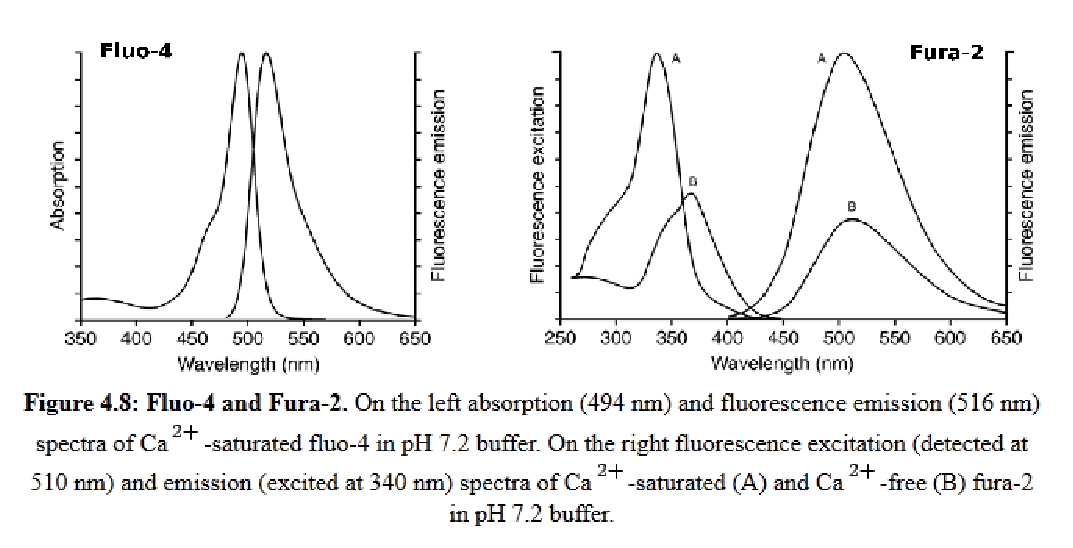
\includegraphics[height=4cm,
    angle=0]{./images/ratiometric_nonratiometric.eps}}
\caption{(A) Non-ratiometric and (B)
ratiometric\footnote{\url{http://www.hexec.it/tesi/node89.html}}}
\label{fig:ratiometric_nonratiometric}
\end{figure}

\subsection{Ratiometric vs. Non-ratiometric}


Another way to classify fluorescent indicators (probes) is its reflection to
wavelengths: ratiometric (dual-wavelength) vs. nonratiometric (single
wavelength) indicators, Fig.\ref{fig:ratiometric_nonratiometric}.

\begin{enumerate}
  \item ratiometric group: Indo-1, Fura-2 (red),  or
  (as long as pH remain constant) SNARF (seminaphtho-rhodafluors)
  \item nonratiometric group: Quin-2, Fluo-3, Fluo-4, $\Ca$ green-2, $\Ca$
  Orange, Rhod-2
\end{enumerate}
Ratiometric indicators have 2 sets of excitation/emission wavelengths. By taking the ratio
of the two fluorescence intensity values taken at two different excitation
wavelength, it allows detecting $[\Ca]$ more accurately, avoiding the effect of
unequal dye loading, bleaching and focal-plane shift. An example is that we have
two cells with the same $[\Ca]_i$, but different dye concentration, so by taking
the ratio, it will reveal that their $[\Ca]$ are identical. Using the ratio
corrects the variation due to unequal dye loading, bleaching. However, due to
the quick binding saturation, it has limited application to measuring a wide
variation of $[\Ca]$.

Non-ratiometric indicators have only 1 pair of excitation/emission wavelength.
Advantage of non-ratiometric indicators is that an increase in fluorescence
signal can be related directly to an increase in $[\Ca]$ and it can measure a
wide range of $[\Ca]$ change. A drawback is that the measured intensity depends
on many factors not related to $[\Ca]$, e.g.
acquisition condition, probe concentration, and optical path length. So, it's
important to emphaisize using the same total dye concentration when using
non-ratiometric dyes, e.g. Fluo-3, Fluo-4.

\subsection{Emission spectra: blue, green, etc.}

Another way is to classify calcium-indicators into several groups
based on the emission spectra:
\begin{enumerate}
  \item blue-emission: Quin-2, Indo-1, Benzothiaza, Fura-2
  \item green-emission: Fura-2, BTC, Fluo-3, Calcium green, Oregon green
  1,2-bis(2-amino-phenoxy)ethane-N,N,N',N'-tetraacetic acid (BAPTA)
  \item yellow, orange-emission: calcium orange, cal- cium crimson, and rhod 2
  \item red and near-infrared emission: calcium crimson and Fura red
\end{enumerate}

\subsection{Chemical form}

Another way of classification is based on their chemical form: salt (acid),
ester, and dextran conjugates.

\subsection{EGTA}

EGTA is an early $\Ca$ indicator. For
calibration, see Sect.\ref{sec:calibrate_EGTA}.

\subsection{BAPTA}
\label{sec:bapta}

BAPTA can binds to $\Mg$ ions, yet to $\Ca$ with $10^5$-fold higher
\citep{tsien1980}.
Recent studies showed that BAPTA have higher affinity to \ce{Zn^2+} (zinc) than
to $\Ca$. The dissociation constant for $\Ca$ binding is $K_d\sim 0.11\mu$M
at 0.1M KCl. The rate constant of $\Ca$ binding is
$k^+ = 500\muM^{-1}.s^{-1}$ ~\citep{pethig1989}.


\subsection{Quin-2 (1980)}
\label{sec:quin-2}

Quin-2 is the first generation non-ratiometric fluorescent $\Ca$ indicator
\citep{tsien1980, tsien1982,tsien1989}. Quin-2 has a single excitation and
emission wave length ($\lambda_{ex}=332$ nm, $\lambda_{em}=498$ nm).
The excitation wavelength $\lambda_{ex}=339$ nm is too short, as a significant
amount can comes from autofluorescence $F_\min$ (i.e. where $[\Ca]=0$). So, this
is a weak point of using Quin-2.

\textcolor{red}{When bound to $\Ca$, the emission fluorescence increase 5-6
fold}.
Quin-2 has a high affinity of $\Ca$, making it work well to measure $[\Ca]_i$ at
resting levels, i.e. near $10^{-7}$M or 0.1$\muM$. \citep{sheu1984} shown the
resting $[\Ca]_i$ in rat ventricular myocyte was about 0.18$\muM$ using with
$K_d = 0.115\muM$  {\it in
  vivo}. 
  
Quin-2 also binds to $\mg$ with $K_d=1-2$mM (low-affinity). In vivo, the
dissociation constant can be different due to the effect of Mg; thus it is
called the effective dissociation  constant, whose value is $K_d = 115$ (nM) (at
$[\Mg]_i=1$ mM). This can be altered by changing $[\Mg]_i$, e.g. $K_d=60$ (nM)
at $[\Mg]_i=0.0$.

Quin-2 also serve as a buffer for $\Ca$. At higher levels, the dye approaches
saturation and lose resolution.
It means that at high $[\Ca]_i$, we need dyes with low $\Ca$-affinity to
measure. Increase in Quin-2 fluorescence indicates an increase
in $[\ca]_i$, without much shifting in emission and excitation wave
length between bound vs. unbound Quin-2).

Newer dyes of choice, with 2 different wave lengths, are Fura-2
(Sect.~\ref{sec:fura-2}) and Indo-1 (Sect.~\ref{sec:indo-1}).  This gave birth
to the quantitative ratio fluorescent techniques $\Delta F=F_a/F_b$. The key
characteristic of these new indicators is the wavelength shift (in either
emission or excitation) upon binding with an ion, e.g. $\Ca$.


\subsection{Fura-2 (1985)}
\label{sec:fura-2}

Fura-2 is a ratiometric fluorescent dye which binds to free intracellular $\Ca$
with 30-fold brighter than Quin-2~\citep{grynkiewicz1985}.
\textcolor{red}{ Newer calcium indicators is Cameleons}
(Sect.~\ref{sec:cameleons}).
\begin{itemize}
\item In the absence of $\Ca$, excitation maximum is 372nm. When bound
  to calcium, the maximum shift is 340nm.

\item In both bound and unbound, the emission wavelength of the Fura-2
  is $\lambda_{em}=510$ nm.
\end{itemize}

So, using the ratio of the fluorescence excited at these two
wavelengths $F_{340}/F_{380}$ is directly correlated to the amount of
free $[\ca]_i$. Recently, they also use
$F_{335}/F_{405}$~\citep{goldhaber1991,chudin1999icd}, as well as
$F_{360}/F_{390}$~\citep{Larbig2010}. However, the emission at 360nm
is closed to the noise floor, so an alternate approach is to use
{\bf ``self-ratio''}. Particularly, only the emission data at 390nm is
used. The inverse of the emission at this single wavelength is
normalized ($\Delta F/F_0$).

Fura-2AM added to the cell is about 0.5$\muM$ \citep{williams1990qic} which
gives level of Fura-2 about 13-27$\muM$.

In chromaffin cells, fura-2 has $k^-_m=97$ (1/s), and $k^+_m=601
(\mu$M$^{-1}$.s$^{-1}$. Fura-2 has a rapid binding kinetics, with the relaxation
time is of the order of 5ms. The dissociation constant for Fura-2 is thus
$K_d=k^-/k^+=0.16\mu$M~\citep{wagner1994erb}.

\citep{blatter1990} measured the diffusion coefficient of Fura-2 is $D_F =
31.9\mum^2/s$.
This value is about 3x lower than the expected value of free diffusion in the
myoplasm. It means that a certain amount of dyes bound to the non-mobile
proteins. Assuming of instantaneous binding, this gave 30-35\% of the Fura-2 are
available for diffusion.
The diffusion of free Fura-2 and Ca-bound Fura-2 are quite similar.

% Depening on the dye, if there are two
% excitation wavelength, then we have two values of R: $R_\min$ (lower wavelength), and $R_\max$ (higher wavelength).

\begin{framed}
  Nikon Diaphot can excite wavelength at 1200Hz, so that both
  wavelengths can be updated at every 800$\mu$s. All fluorescence data
  are filtered with a 50Hz lowpass Gaussian filter (Clampex 9).
\end{framed}




% \subsection{Fura-2AM}
% \label{sec:fura-2am}


\subsection{Indo-1 (1985)}
\label{sec:indo-1}

Indo-1 is a ratiometric indicator synthesized by Tsien
group~\citep{grynkiewicz1985}.
It has about 30-fold brighter than Quin-2, which means the affinity to $\Ca$ is
high, i.e. a small change in $[\Ca$ can be easily detected using a smaller
amount of dyes, and thus avoid the buffering effect of the dye on $\Ca$.
Indo-1 is different from Fura-2 in that it has dual emission peak, rather than
dual excitation peak. 

\begin{itemize}
\item The main emission peak, in $\Ca$-free solution, is 485nm; while
  in $\Ca$ solution, it shifts to 405nm. Some uses a slightly different
  wavelength, e.g. 400/475. Fluorescence emitted by the cell was recorded as
  photon counts per second at 405 and 485 nm, i.e. $F_{405}$ and $F_{485}$. The
  illumination field was restricted to a circular spot 30$\mu$m in diameter. The
  background fluorescence recorded from a field of the same size at both
  wavelengths was subtracted from the signal recorded, e.g.
  $R_{405}=F_{405}-\text{background}$ and $R_{485}=F_{485}-\text{background}$,
  before the fluorescence ratio $R=R_{405}/R_{485}$ was computed.

\item In both bound and unbound state, the excitation wavelength of
  Indo-1 is 365nm \citep{grynkiewicz1985}. Newer samples use a different
  wavelength, e.g. 353nm by \citep{}
\end{itemize}
\citep{blatter1990} measured the diffusion coefficient $D_F = 15.7\mum^2/s$.
\citep{westerblad1996} measured $K_d = 311$ (nM) and resting calcium in Xenopus
muscle is 0.052$\muM$. 

\begin{framed}
Indo-1 is more pH-insensitive than EGTA between pH 6.0 and 8.1, and has high
selectivity to $\Ca$ than other ions ($\Mg, \Zn, \Mn$). Similar to Fura-2,
Indo-1 is not cell permeable. However, Indo-1AM is membrane-permeable.
\end{framed}

The main disadvantage of Indo-1 is that it has rapid photobleaching under UV
illumination, which generate $\Ca$-insentive fluorescent compount from Indo
whose emission spectrum is very closed to $\Ca$-free Indo-1. Also,
autofluorescence due to NADH also overlap with the spectrum of $\Ca$-free
Indo-1 \citep{takahashi1999}.


Many {\it in vivo} methods estimate the {\it in vivo} values of
minimum and maximum fluorescence ratios ($R_{min}, R_{max}$) and using
an {\it in vitro} dissociation constant $K_d$.
\begin{itemize}
\item $R_{min}$ is hard to measure reliably as it's difficult to get
  $[\ca]_i$ to a very low level ($< 1$nM).
\item $R_{max}$ is also hard to measure reliably in cardiac myocytes
  as the high concentration cause massive hypercontracture of the
  cell, which can destroy cellular integrity.
\end{itemize}

\begin{framed}
  {\it In vivo} measurement of $R_{min}$~\citep{bassani1995a}:
  \begin{itemize}
  \item indo-1 loaded cells were exposed to 10 mM caffeine twice, to
    empty SR $\Ca$ stores, then superfused with 0Ca solution for 15min
  \item bath solution was then switched to K-buffer containing 5 mM
    EGTA, leaving for 20min perfusion
  \item
  \end{itemize}
{\it In vivo} measurement of $R_{max}$
\end{framed}


\subsubsection{Finally}
\label{sec:finally}

\begin{equation}
  \label{eq:966}
  [\ca]_{i,tot} = [\ca]_i + \frac{B_{max1}}{1+(K_1/[\ca]_i)}+
  \frac{B_{max2}}{1+(K_2/[\ca]_i)}+ \frac{[\text{indo}]_i}{1+(K_{in}/[\ca]_i)}
\end{equation}
with $B_{max1},B_{max2},K_1,K_2$ are empirical constants for
buffering. The last term reflects $\Ca$ bindings to indo-1,
i.e. $[\text{indo}]_i=50 \mu M$, $K_{in}=250 nM$. To obtain the rate
of transport, we differentiate it
\begin{equation}
  \label{eq:967}
  \frac{d[\ca]_{i,tot}}{dt} = J_{sr}+J_\ncx+J_{slow}-J_\leak
\end{equation}

The fluxes can be described using simple quasi-empirical $[\ca]$
dependent of the form
\begin{equation}
  \label{eq:968}
  J_x = \frac{v_{max}}{1+(K_m/[\ca]_i)^n}
\end{equation}
with $v_{max}$ is the maximum flux rate, $K_m$ is Michaelis-Menten
constant, $n$ is Hill coefficient. and then fitted with experimental
data to find the parameters~\citep{bassani1994rir}.


\subsection{Fluo-2 (1988)}
\label{sec:fluo-2}

The {\it in vitro} $K_{d,\ca} = 390$ nM for Fluo-2AM (measured at 20$^\circ$C,
in quart capillary tubes filled with Fura-2 solution, sealved by Vaseline at
each end \citep{baylor1988})\citep{hagen2012}. There're evidences that in
myoplasm of frog skeletal muscle fibers, the diffusion constant is 3-fold
smaller than expected on the basis of the molecular weight \citep{baylor1988},
which suggests a majority of Fura-2 molecules bind to protein. The {\it in vivo}
$K_d = ???$ can be estimated using least-square fitting \citep{konishi1988}.
\begin{equation}
K_d = \frac{F-F_\min}{F_\max-F}[\Ca]
\end{equation}
with $F_\max, F_\min$ are fluorescence intensities measured at zero $[\Ca]$
(EGTA solution), and saturating $[\Ca]$, respectively. This can also be derived
from the fomula
\begin{equation}
K_d = K_{d,\ca}(1 + \frac{[\Mg]}{K_{d,\Mg}})
\end{equation}
with $K_{d,\ca}$ is the dissociation constant for $\Ca$ in the absence of $\Mg$,
and  $K_{d,\Mg}$ is the dissociation constant for $\Mg$ in the absence of $\Ca$.
The normal concentration of $\Mg$ in the cytosol is about 1.5mM. This gives the
$K_d=188$nM in vivo. \citep{minta1989} estimated effective $K_d=0.37\muM$. 

The dissociation constant $K_{d,\Mg}=1.9$mM.

\begin{framed}
The Fluo family share a common molecular structure: a BAPTA-like $\Ca$-binding
site linked covanlently to a xanthene moiety. It also shows an increase in
cellular loading efficiency, reduced pH sensitivity, and the excitation maxima
that match the emission wavelength of common lasers \citep{hagen2012}.
\end{framed}


\subsection{Fluo-3 (1989)}
\label{sec:fluo-3}

Fluo-3 is a nonratiometric indicator discovered by Tsien
group~\citep{minta1989,kao1989} from BAPTA combined with a fluorescein-like
structure. The excitation and emission wavelengths are $\lambda_{ex}=506$ nm,
$\lambda_{em}=526$ nm.
The freeform excited wavelength (448nm) make Fluo-3 producing little
autofluorescence and thus inducing less photodamage in dye-loaded cells than
previous dyes. So, it's suitable for use in flow cytometry, confocal laser
scanning microscopy, microplate screening assays, or light microscopy.


Fluorescence of $\Ca$-bound fluo-3 has about 40x-200x more intensity than its
$\Ca$-free counterpart~\citep{harkins1993} making it the most widely used dye in
detecting $[\Ca]_i$, yet it's quite suceptible to photobleaching than many other
indicators.
As the increase in $[\Ca]_\myo$ is in the range of 5x-10x, Fluo-3 is good enough
to detect these changes.
This yields a high $F_\max/F_\min$ ratio making it superior in detecting local
$\Ca$ elevations, than Fura-2 and indo-1.

% \begin{framed}
%   Fluo-3 is unsuitable for two-wavelength ratiometric,
%   i.e. $R_\max/R_\min$. Ratiometric measurements can be made using Fura red, or
%   (as long as pH remain constant) SNARF (seminaphtho-rhodafluors).
%   However, it has high $F_\max/F_\min$ which
%   produce high signal contrast and high signal-to-noise ratio, making
%   Fluo-3 is superior to Fura-2 or Indo-1.
% \end{framed}


Fluo-3 is a penta-valent anion (mol wt 765) and is predicted to have a
\textcolor{red}{ diffusion coefficient of $90\mu m^2/s$}.
However, in skeletal muscles, the diffusion was measured between 12 to 30 $\mu
m^2/s$~\citep{harkins1993}, suggesting that about 80\% of the dyes  bound to
immobile cellular constituents ~\citep{smith1998}. Experimental results showed
the evidence that fluo-3 interact with large molecular weight proteins, e.g.
aldolase. So, computational models either (1) use small diffusion constant, (2)
use real diffusion constant and consider mobile Fluo-3 and immobile
protein-bound Fluo-3 explicitly in the model.

Fluo-3AM added to the cell is about 2$\muM$ \citep{williams1990qic} which
results into total [Fluo-3] $\sim 50\muM$.

With the presence of proteins in the myoplasm, it also affect the $K_d$ with
calcium. In vitro $K_d$ was measured using various solutions of known $[\Ca]$,
created by mixing 4mM EGTA and 4mM Ca-EGTA in various ratios \citep{mcguian1991,
zhao1997}. The dissociation constant with $\Ca$ {\it in vitro} is $K_d=325$nM
(or $\approx 335$
nM\footnote{\url{http://www.invitrogen.com/1/1/604-fluo-3-am-cell-permeant-special-packaging.html}}
or 390
nM\footnote{\url{http://www.embl.de/eamnet/html/calcium/nonratio.htm}}\citep{hagen2012}
or $K_d=400$nM \citep{trafford1999nrr}). \citep{minta1989} estimated effective
$K_d = 0.4\muM$

{\it In vivo}, the calcium-affinity is becoming lower, i.e. higher dissociation
constants. \citep{smith1998} estimated it to be $K_d\sim
1.13\muM$. Recent measurement showed $K_d=0.8\muM$ \citep{hagen2012}, or
$K_d=0.89\muM$ measured on rabbit cardiac myocytes \citep{loughrey2003} (i.e.
$k^+=80\muM^{-1}.s^{-1}, k^-=72.s^{-1}$).

\begin{framed}
The cytoplasmic environment also alters the interaction with calcium, i.e.
slowing both the dissociation constant and association rate. In particular, $k^- = 200-700 $ per second
\citep{eberhard1989} to 90 (per second) \citep{harkins1993}; $k^+=1000
\muM^{-1}.s^{-1}$ {\it in vitro} to 80 $\muM^{-1}.s^{-1}$ {\it in vivo}. This
eventually increase $K_d$ from 0.4$\muM$ (in vitro) to 1-3$\muM$ (in vivo).
\end{framed}

The cell is stimulated using field stimulation (e.g. Voltage-clamp 25-30V for
2.0ms) or by current-injection (I-clamp 2nA for 2.0ms). In patch-clamp
experiment (i.e. AP or current clamp), the elapsed time between 10\% rise and
90\% decay, known asn APD90, and the $t_{90-10}$ the time required for the
calcium transient (CaT) to decay from 90\% to 10\% of the peak amplitude, are
\citep{hagen2012}
\begin{itemize}
  \item APD90 = 38.6$\pm 2$ms, first transient $t_{90-10}=599\pm 42$ms, and
  steady-state $t_{90-10}=631\pm 29$ms  (Fluo-4)
  \item APD90 = 39.2$\pm 1.6$ms, first transient $t_{90-10}=415\pm 24$ms, and
  steady-state $t_{90-10}=426\pm 24$ms (Fluo-3)
  \item APD90 = 37.0$\pm 1.0$ms, first transient $t_{90-10}=777\pm 40$ms, and
  steady-state $t_{90-10}=682\pm 40$ms   (Fluo-2)
\end{itemize}
In rat ventricular myocyte, the average volume was 36.8pL/cell, and cytosolic
fraction is 0.65 \citep{bers2001ecc}. At high stimulation rate (1Hz vs. 0.5Hz),
there's an increase in fluorescence baseline (F0) in Fluo-2 and Fluo-3, but not
in Fluo-3.



\subsubsection{Cordeiro et al. (2001) - Rabbit heart Purkinje fiber}
\label{sec:cordeiro_2001}

\citep{cordeiro2001} used confocal microscopy (Bio-Rad 1024 laser-scanning confocal
microscope) and 100$\muM$ Fluo-3.

Staining with 5$\muM$ di-8-ANEPPS dye, the results shown that Purkinje fibers
lack T-tubular structure. The calcium was modelled binding to ATP, Fluo-3 and
Troponin (Trpn). The cell was modeled as a cylinder divided into 100 concentric
compartments to allow diffusion equations of $\Ca, \Mg, \ATP$ and Fluo-3. The
rate constants for $\ATP$ binding was based on \citep{baylor1998}, adjusted to
36$^\circ$C with $Q_{10}=2.0$. Other diffusion constants: $D_\Ca= 300 \mum^2/s$
and $D_F = 25\mum^2/s$.  The total concentration of buffers, as claimed by the
authors unknown at that time, so they were fitted to experimental data by
adjusting the concentration of [Trpn], [ATP], and [Fluo-3].

They estimated peak F/F0 reached $\sim 2.0$ at the surface and $1.75$ at the
center.

\subsubsection{Inoue - Bridge (2003) - rabbit ventricular myocytes}
\label{sec:Inoue-Bridge_2003}

\citep{inoue2003} (Sect.\ref{sec:spark_Inoue-Bridge_2003}) used BioRad MCR-1024
laser scanning confocal microscope, and Fluo-3. Images were captured with
0.15$\mum$ and 2ms per pixel resolution.

Under AP stimulus, spark appearances are litmited to the beginning of APs. After
treatment with 1$\muM$ thapsigargin, the sparks disappear.

The peak F/F0 values are greater than 1.5.  The FWHM spark size were 1.8$\mum$
(in mice), and $2\mum$ (in rats).



\subsection{Calcium Green-1 (CG-1)}
\label{sec:Green-1}
\label{sec:CG-1}

Calcium Green-1 (two wavelengths: 506/531 nm) can increase intensity up to
14-fold upon $\Ca$ binding, with little shift in wavelengths.
Although Calcium Green-1 is structurally similar to Fluo-3
(Sect.\ref{sec:fluo-3}, it is more fluorescent at low calcium concentrations,
facilitating the determination of baseline Ca2+ levels and increasing the
visibility of resting cells, i.e. $K_d = 315$ nM.

The probe is excited by visible light, as the energy required for excitation is
low, which means less photodamage for cell. Commonly used laser-based
instruments (i.e., confocal laser scanning microscopes) are able to efficiently
excite these indicators, and their emissions are in regions of the spectrum
where cellular autofluorescence and scattering backgrounds are often less of a
problem.

\subsection{Cameleons (1997)}
\label{sec:cameleons}

Cameleons are genetically-encoded calcium indicators.

\subsection{Rhod 2 (1989)}
\label{sec:rhod_2}

\citep{minta1989} developed Rhod2. Rhod 2 is used to measure mitochondrial
$\Ca$. As the mitochondrial membran exihibits a large potential difference, the
AM form of Rhod2 can be easily injected into the mitochondria membrane.
Effective dissociation constant $K_d=1.0\muM$ \citep{minta1989}.

\subsection{Fura-red (1989)}

Fura-red is chemically similar to Fura-2, but the absorbance and
fluorescence-excitation band is in visible, not ultra-violet, wavelengths
\citep{demarinis1990}. Fluorescence excited with 2 wavelengths: 420nm and 480nm
(using Lens 32x, N.A.=0.60) after noise correction are $F_{420}, F_{480}$.
The fluorescence emission at wavelength greater than 550nm was selected with a
barrier filter. The ratio $R=F_{420}/F_{480}$ is calculated. The values of R for
the calcium-free and Ca-bound forms of the indicator are denoted as $R_\min,
R_\max$.

Based on Sect.\ref{sec:in_vitro_measure_Fluo}, parameters for {\it in vitro}
measurements are:
\begin{enumerate}
  \item At buffers 2.0cP (no aldolase): (1) 420nm excitation: $Y_1=1.050$
  (Calcium-free), $Y_1=1.122$ (Calcium-bound); (2) 480nm excitation: $Y_1=1.100$
  (Calcium-free), $Y_1=1.037$ (Calcium-bound).
  \item At bufers 1.6cP (with aldolase): (1) 420nm excitation: $Y_1=1.038$
  (Calcium-free), $Y_1=1.106$ (Calcium-bound); (2) 480nm excitation: $Y_1=1.101$
  (Calcium-free), $Y_1=1.033$ (Calcium-bound).
\end{enumerate}

The dissociation constant $K_d$ was estimated using the least-square fit for the
equation, assuming 1:1 binding of calcium
\begin{equation}
\label{eq:mc154}
f = \frac{[\Ca]}{[\Ca]+K_d}
\end{equation}
with $f$ is the fraction of calcium-bound fluorescence. This gives {\it in
vitro} $K_d = 0.41\muM$.

Fura-red has been used in measuring free-calcium in frog skeletal muscles
\citep{kurebayashi1993}, with [Fura-red] = 25$\muM$.
% $\ge$ 0.2-0.3mM.
To estimate free calcium, first they map R to $f$, and then using equation
\ref{eq:mc154} with a given value of $K_d$ to find $[\Ca]$.


\subsection{Fluo-4 (2000)}
\label{sec:fluo-4}

Fluo-4 is an improved version of Fluo-3 (Sect.\ref{sec:fluo-3}), with
freeform excited wavelength is higher $\lambda_{ex}= 488$ nm, which provides
brighter fluorescence emission.
The wavelengths in $\Ca$-bound form are ($\lambda_{ex}=494$ nm,
$\lambda_{em}=516$ nm).

Fluo-4 is similar to Fluo-3 in several ways, e.g. spectral properties,
stability, $K_{d,(\Ca)}$, convenience and ease of loading, and high $\Ca$-
dependent fluorescence enhancement \citep{gee2000}.
It is often used in the form of Fluo-4AM so that can be inserted into the cell
via diffusion. However, using AM ester form, it leads to significant organellar
compartmentalization in Fluo4-AM than in Fluo3-AM \citep{hagen2012}.

The {\it in vivo} dissociation constant was estimated about $K_d=9.7 \muM$
\citep{} or $K_d = 1.400\muM$ \citep{hagen2012}.


Fluo-4 can quantify $[\ca]_i$ in the range 100nM to 1$\mu$M.
{\bf In vitro} dissociation constant is about $K_d=350$nM \citep{hagen2012}. Due
to its higher fluorescence emission intensity, we can use a lower amount of
Fluo-4, compared to Fluo-3, to measure intracellular $\Ca$ concentration.

\begin{framed}
Fluo-4FF is Fluo-4 related dyes that have lower $\Ca$-affinity so
that can measure $[\ca]$ at higher level and wider range (from 1$\muM$ to 1 mM).
Fluo-4FF can excite under argon-ion laser source with $\lambda_{ex}=488$ nm. In
$\Ca$-bound  form, $\lambda_{ex}/\lambda_{em}=494/516$ nm.
\end{framed}

\begin{figure}[hbt]
  \centerline{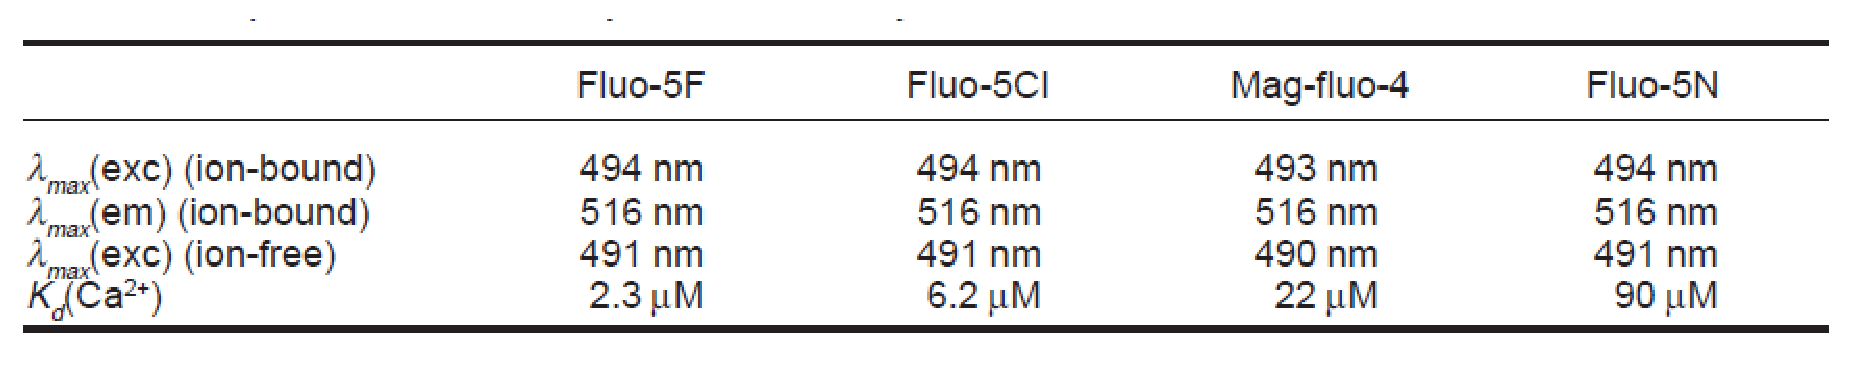
\includegraphics[height=2.2cm,
    angle=0]{./images/fluo-4_lowaffinity.eps}}
\caption{Low-affinity $\Ca$-indicator dyes: Fluo-5F, Fluo-5Cl,
  Mag-fluo-4, Fluo-5N}
\label{fig:low-affinity}
\end{figure}

The data is captured using Omega Optical bypass filter (Brattleboro, VT, USA).
Images were acquired with Quantix HCCD camera. The images were then analyzed
using MetaFluor imaging software (Universal Imaging Corp, PA, USA). A normalized
fluorescence image is generated: (1) each image was 'background-corrected' by
pixel-by-pixel subtraction of the average measured value from a sampled
extracellular region, (2) the background-corrected fluorescence image was then
normalized, pixel by pixel, to the fluorescence masured in a single image from
the initial control conditions (to subtract autofluorscence)


\subsection{Oregon Green BAPTA}
\label{sec:Oregon-Green-BAPTA}

Oregon Green 488 BAPTA-1 is a fluorescent dye $\Ca$ indicator, with two
wavelengths 494/523 nm. It can detects $\Ca$ increase upto 14 fold.

\subsection{GFP-based $\Ca$ indicators}
\label{sec:GFP_dye}

Green fluorescent protein (GFP) is a protein composed of 238 a.a residues
(26.9kDa) from jellyfish {\it Aequoria victoria} that exhibits blight green
fluorescence when exposed to light in the range of wavelength from blue to
ultraviolet. GFP-based forms are used as biosensors, e.g. a reporter of gene
expressions. Half-life of GSP was estimated to be $\tilde 26$ hours.

PROS: it can be introduced into the cells and maintained in the genome through
breeding.



\subsection{-- GCaMP: GCaMP6}
%\subsection{GCaMP6}
\label{sec:GCaMP6}

GCaMP is a fusion of GFP, calmodulin and M13, that is used as a calcium
indicator with a good signal-to-noise. The widely use is in neurons, where
calcium can bind to calmodulin (up to 4 calcium ions per calmodulin).
The highest performance GCaMP are GCaMP3 \citep{tian2009} and GCaMP5 of faster
kinetics and greater response than the original GCaMP.

GCaMP6 has been introduced since 2013 (Chen et al., 2013) which has been shown
to outperform other sensors in cultured neurons and in zebrafish, flies, and
mice {\it in vivo}.
\begin{itemize}
  \item layer 2/3 pyramidal neurons of the mouse visual cortex

GCaMP6 reliably detected single action potentials in neuronal somata and
orientation-tuned synaptic calcium transients in individual dendritic spines.
  
  \item 
\end{itemize}

\subsection{Fluo 5N}
\label{sec:fluo5N}

Fluo-5N is used to measure $[\Ca]$ in the SR which was pioneered by Bers and
colleagues \citep{shannon2003,shannon2003cs}.
To calibrate $[\Ca]_\SR$ from the fluorescence intensity, \citep{shannon2003}
suggested the formula for {\it in situ} calibration
\begin{equation}
\Delta [\Ca]_\sr = K_d \frac{1+\frac{\Delta
F}{F_0-F_\min}}{K_d/C_0-\frac{\Delta F}{F_0-F_\min}}-C_0
\end{equation}
with $F_0$ and $F_\min$ is the fluoresence level at rest, and after emptying SR,
respectively. With Fluo-5N, $K_d = 400\muM$, and diastolic $[\Ca]$ is
$C_0=1.0\mM$ .


Fractional change in CSQN-bound $\Ca$ is calculated as
\begin{equation}
\Delta [\text{CaCSQN}] = K_{d,\CSQN} \frac{\Delta
[\Ca]_\sr}{C_0(K_{d,\CSQN}+[\Ca]_\sr)}
\end{equation}
with $\Ca$ dissociation constant of CSQN: $K_{d,\CSQN}= 500\muM$.




\subsection{Citrate and Maleate and ADA}
\label{sec:citrate-maleate}

Citrate is a weak acid, can be used as $\Ca$ chelating agent
($K_d=0.47$mM). Maleate has $K_d=11$mM). They can be effectively
transported into the SR, thus increasing $\Ca$ buffering capacity of
the SR.

They are diffusible exogenous buffers.

\subsection{Asante Calcium Red (ACaR)}

Asante Calcium Red (ACaR) is a new ratiometric $\Ca$ indicator. 

\subsection{Fluorescence in myoplasm vs. nucleoplasm}

It has been shown that Fluo-3 and Fluo-4 have distinct characteristics in the
cytoplasmic vs. nucleoplasmic compartment \citep{thomas2000}. Some studies
reported the leak of indicators from the cytoplasm to the extracellular medium
via sarcolemmal anion transporters \citep{mcdonough1989,mitsui1993}.

\section{-- Protein-based calcium indicator}
\label{sec:calcium-indicator-protein-based}

Protein-based genetically encoded calcium indicators (GECIs) is another
breakthrough come from Roger Tsien (Miyawaki et al., 1997).

Early GECIs are not powerful due to slow response kinetics and low
signal-to-noise ratios.



\section{Buffers (in vitro + in vivo) and Dyes Properties}
\label{sec:buffers-dyes}

\subsection{Buffers alone (in vitro)}

The standard buffer solution contained (in mM) \citep{kurebayashi1993}: 97.7
KCl, 10 PIPES (piperazine-NN'-bis[2-ethane-sulfonic acid]) and either 10 EGTA
('0 $\Ca$' solution) or 10 \ce{CaCl2} ('sat. $\Ca$' solution). The ionic
strength was 0.15 M and, unless indicated otherwise, had a pH of 7.03. [Note:
all solutions were titrated to a pH of 7.00 at room temperature (-200C). At 16C,
a solution pH of 7.03 is expected, given the temperature dependence of the PIPES
buffer (38)].
For the experiments that characterized the effects of $\Mg$  on fura red, 10 mM
\ce{MgCl2} was added to the 0 and sat. $\Ca$ solutions, resulting in free
[Mg2+]'s of approximately 8.3 and 10 mM, respectively (assumed apparent
dissociation constant of EGTA for $\Mg$, 40 mM); KCl was lowered to 67.7 mM to
maintain ionic strength at 0.15 M.
\begin{itemize}
  \item To characterize the effect of pH on Fura red, pH was changed to 6.8
  (titrated with HCl) or 7.5 (titrated with KOH). Accordingly, KCL was changed
  to 100 mM and 93.3 mM, to maintain ionic strength  (due to the effect
  of PIPEs to total ionic strength).
\end{itemize}

The viscosity in buffer alone is 1.1cP.

\subsection{Buffers + sucrose (viscosity or diffusion)}

The effect of viscosity on the indicator should be studied in buffer plus
sucrose, which increase the viscosity (reported in centipoise = cP) from 1.1cP
(no sucrose) to 2.0cP (with 0.564M sucrose), and 2.9cP (with 0.842M sucrose)
\citep{kurebayashi1993}.

\subsection{Buffers + aldolase}

Aldolase is the most abundant soluble proteins in myoplasm on a weight basis
\citep{ottaway1977}. Early papers used rabbit aldolase \citep{kurebayashi1993}
which is added to the buffer in the amount of 55 mg/ml protein, giving the
solution viscosities 1.6 cP. Protein solutions were used either immediately
after dialysis or stored frozen at -20$^\circ$C and used within 3 days.

The effect of aldolase was tested with different concentration e.g. 0, 15, 30
and 55 mg/ml while keeping the viscosity the same (1.6cP) by adjusting sucrose
amount.


\subsection{Dissociation constant $K_d$ of the dyes}
\label{sec:Kd_dyes}

An important quantity to reflect the property of the dye is the dissociation
constant $K_d$. The value of $K_d$ is dependent upon pH, temperature, viscosity,
ionic strength, protein binding and the amount of $\Mg$, as well as other metal
ions.
\begin{enumerate}
  \item The $K_d$ reported from the product website for the dyes are based on {\it in
vitro} environment. A typical {\it in vitro} environment is simple salt solution
(150mM KCl, 1mM $\ce{MgCl2}$, with pH $\sim 7$, and possibly with sucrose added
to approximate the viscosity of the cytosol (in muscle, this is about twice of
that in a simple salt solution)) \citep{baylor2000}.

 \item The {\it in vivo} (intracellular) environment afffect strongly on
 indicator properties ($k^+,k^-$) and increase $K_d$. \textcolor{red}{The
 dissociation constant $K_d$ reported in this book is  based on {\it in vivo}}
 (i.e. with the presence of $\Mg$ and other metal ions).
\end{enumerate}

Concentration of free $\Mg$ in cytosol is about 1,000- to 10,000 fold higher
than free $[\Ca]$. Thus, using a calcium indicator with high selectivity over
$\Mg$ is better than using the one with lower selectivity to avoid the
interference of $\Mg$ to the precised measurement. In vivo, the adding of
soluble proteins can affect at least 2 parameters:
$F_\min$ (i.e. the value of fluoresences in Ca-free solution) and $K_d$. E.g.
adding 55mg/ml soluble protein, with Fura-2, $F_\min$ increase 90\%, and $K_d$
incrase 3.6 fold (from 0.19 to 0.69$\muM$).

Many studies suggested as much as 85\% of fluorescence is protein-bound, giving
the change in $K_d$ up to 5-fold, e.g. Fura-2 \citep{konishi1988},
\citep{thomas2000}.


The time constant at equilibrium for a 1:1 binding is defined as
\begin{equation}
1/\tau = k^+ [\text{Buffer}_{total}]
\end{equation}

The value of $K_d$ in intact myocyte can be estimated using the suggested
formula \citep{loughrey2003}
\begin{equation}
K_d = \frac{(F_\max-F_\text{dia})[\Ca]_\text{dia}}{F_\text{dia}}
\end{equation}
with $dia$ refer to the case with minimum fluorescence. 



\subsection{Diffusion constant of the dyes}
\label{sec:dye_diffusion}

Giving the free diffusion coefficient is $D$, and the ratio of bound-fluoresence
over free fluorescence $R=$(dye-bound)/(dye-free). Then, the effective diffusion
constant is
\begin{equation}
D_\app = \frac{D}{1+R}
\end{equation}

The ratio measured at ver low $[\Ca]$ is $R_\min$, and very high $[\Ca]$ is
$R_\max$.



\section{Estimate $[\Ca]$: Calibrate Fluorescent signal}
\label{sec:calibrate_Fluo}
\label{sec:estimate-Ca}

Review: \citep{takahashi1999,thomas2000, baylor2000, guatimosim2011}.

Fluorescence dyes is a powerful indicator to detect the level of free $[\Ca]_i$
in the cytosol~\citep{baylor2010} or sarcoplasmic reticulum. The most
straightforward approach is to determine in-situ calibration curves. Here, the
effective dissociation constant $K_d$ is of particular important and $K_d$ must
be compatible with the $[\Ca]$ in the range of interest. Typically, the dyes can
detect $[\Ca]$ in the range of $0.1K_d$ to $10K_d$.

\begin{framed}

IMPORTANT: $K_d$ of the dye depends on many factors: pH, temperature, ionic
strength, viscosity, protein binding and the presence of $\Mg$, and other ions.
All $\Ca$ indicators are also $\Ca$ buffers. So, unavoidably, the measurement of
$\Ca$ concentration with indicators leads to an increase in the $\Ca$ buffering
capacity.

$K_d$ measured in vitro is well-defined but is not the same as actual $K_d$ in
the cell. The reason is that in the cell, there are many factors that affect
$K_d$, e.g. pH, viscosity, ionic strength. So, $K_d$ for the same dye can be
different between different cell types in vivo. Recently, \citep{hagen2012} did
a study on the properties of different dyes (Fluo-2, Fluo-3 and Fluo-4). $K_d$
measured in a protein-rich buffers like the cytosol were significantly higher
than that in simple buffers i.e. a decrease in $\Ca$ affinity.
\end{framed}

Some studies have suggested that as much as 85\% of the cytosolic $\Ca$
indicator bind to protein, which could increase the dissociation constant $K_d$
upto 5-fold \citep{thomas2000}. Other causes can be the indicator
unintentionally loaded into other compartment, e.g. up to 50\% of the
fluorescent $\Ca$ indicator can be found in the mitochondria. Most dyes
(fluorescence) are assumed to react with $\Ca$ according to a 1:1 binding
reaction
\begin{equation}
  \label{eq:990}
  \ce{Ca^2+ + D <=>[][K_{e,\ca}] CaD}
\end{equation}
with $K_{d,\ca} = \frac{k_{off}}{k_{on}}$ the dissociation constant of the
indicator for $\Ca$.
\begin{enumerate}
  \item  {\it In vitro} value of $K_{d,\ca}$ is often measured in
the absence of $\Mg$ (0.1-0.1M salt solution at $T=6-22^\circ$C, pH$\sim$7). So,
$[D]_T=[D]+[\text{CaD}]$.
	\item {\it In vivo}, the metal binding site of the indicators can also react with
$\Mg$ with an appreciable affinity, so for a more realistic modelling, depending
on  the dyes being  used, we  may consider this effect in the system
(Sect.\ref{sec:fluorescence-dyes}). Then the total dye is $\Dt=
[D]+[\CaD]+[\MgD]$. If we consider $\Mg$ explicitly in the model, we may use the
in vitro $K_d$. Otherwise, we may need to use a different value for $K_d$ in the
simulation which is higher than that being shown on the product website.
\end{enumerate}

\begin{equation}
  \label{eq:991}
  \ce{Mg^2+ + D <=>[][K_{d,Mg}] MgD}
\end{equation}

The choice of calibration is dependent (1) the dye is ratiometric or
nonratriometric, (2) in vitro or in vivo (in situ). \textcolor{red}{REMEMBER:
Before performing any calculation below, the fluorescence level CaF need to be
deconvoluted from the fluroescence image to get the pure CaF}.

Under the assumption of rapid equilibrium, the observed fluorescence F is
calculated as follows
\begin{equation}
\F = \F_\max\frac{[\Ca]_i}{[\Ca]_i + K_d}
\end{equation}
with $\F_\max$ is the maximum fluorescence. In many works, $\F_\max=\F_{sat}$
(is assumed to be the fluorescence at saturation $[\CaF]_{sat}$). In
\citep{trafford1999nrr}, $\F_\max$ is measured directly by damaging the cell
with patch pipette. This results in an abrupt increase of $[\Ca]_i$ and saturate
the fluorescence. In the subsections, we will discuss how free calcium is
estimated from fluorescence level, depeneding upon which kinds of dyes are being
used.

\subsection{Ratiometric indicators}
\label{sec:calibrate_ratiometric_indicator}

Define $R$ is the ratio of the two intensity, $R=F_{\lambda_1}/F_{\lambda_2}$.
The use of the ratio automatically cancel out the confounding variables (e.g.
local differences in Fura-2 concentration or cell thickness that may lead to
artifacts). The main disadvantage is that when auto-fluorescence is significant,
we need to subtract the background before doing the ratio. Auto-fluorescence is
significantly reduced in new dyes, so we don't need to do the subtraction step.

\begin{framed}
How to measure ratiometric fluorescence signal?
\begin{enumerate}
  \item Capture the 2 emitted images: one at $\lambda_1$ and $\lambda_2$, say we
  have image R1 and R2
  \item Capture the 2 background images (due to auto-fluorescences): capture the
  background ($\Ca$-free environment) with illumination at $\lambda_1$ and
  $\lambda_2$, say we have images B1 and B2
  \item Take the ratio of the two pictures with background subtraction:
  (R1-B1)/(R2-B2). This is the final fluorescence image (line-scan image).
\end{enumerate}
For new dyes, we can assume $B1=B2=0$.
\end{framed}

Even the methods described below was developed for Fura-2 and Indo-1, they can
be used for other dyes.

\subsubsection{Fura-2}
\label{sec:calibrate_Fura-2}

There are different proposed formula. \textcolor{red}{The first} and widely used
method was derived by ~\citep{grynkiewicz1985}. At rest, we have 
$R_r=F_{420}/F_{480}$; and
action potential stimulation 
$R'=\frac{F_{420}+ \Delta F_{420}}{F_{480}+\Delta F_{480}}$. For ratiometric
measurement and {\it in vitro}, we use
\begin{equation}
[\Ca] = \beta \times K_d \times \frac{R-R_\min}{R_\max-R}
\end{equation}
with $K_d$ is {\it in vitro} dissociation constant. $F$ is the experimentally
measurement intensity (CaF). The subscript $\min$ refers to values measured in
the absence of $\Ca$. The subscript $\max$ refers to values measured at
saturation of $\Ca$ (very high). 
$\beta$ is the ratio of the fluorescence intensities at the wavelength chosen
for the denominator of R in zero and saturating $\Ca$. The value of $R_\max$ and
$R_\min$ can be obtained using low concentration of the dye because the ratio is
theoretically independent of the dye concentration. 


\textcolor{red}{How to come up with the above formula?}: At first, the
fluorescent ratio $R=F_1/F_2$ is defined as 
\begin{equation}
  \label{eq:1288}
  R = \frac{S_{f1}+S_{b1}\frac{[\Ca]_i}{K_d}}{S_{f2}+S_{b2}\frac{[\Ca]_i}{K_d}}
\end{equation}
and then free calcium is derived using
\begin{equation}
  \label{eq:1289}
  [\Ca]_i = K_d\left(\frac{R-(S_{f1}/S_{f2})}{(S_{b1}/S_{b2}-R)}\right)\left(\frac{S_{f2}}{S_{b2}}\right)
\end{equation}

Rationing the fluorescence intensity of the calcium-bound dye and calcium-free
dye, $F_{\lambda_1}$ and $F_{\lambda_2}$ respectively, can yield a good
measurement of $[\Ca]_i$, which is independent of dye concentration and optical
path length (these are uncontrollable parameters).
\begin{itemize}
\item $F_{\lambda_1}$ (or $F_1$) is the fluorescence intensity at wavelength
  $\lambda_1$
\item $F_{\lambda_2}$ (or $F_2$) is the fluorescence intensity at wavelength
  $\lambda_2$
\end{itemize}
The 2 above quantities are determined using the following 4 proportionality
coefficients:
\begin{itemize}
\item $S_{b1}, S_{b2}$ are the fluorescence intensity for $\Ca$-bound dye at
wavelengths $\lambda_1$ and $\lambda_2$, respectively
\item $S_{f1}, S_{f2}$ are the fluorescence intensity for $\Ca$-free dye at
wavelengths $\lambda_1$ and $\lambda_2$, respectively
\end{itemize}
E.g.: For Fura-2, then $S_{f2}/S_{b2}=$[Fura-2]/[Ca.Fura-2].
\begin{equation}
  \label{eq:1286}
\begin{split}
F_1 = S_{f1}c_f + S_{b1}c_b \\
F_2 = S_{f2}c_f + S_{b2}c_b
\end{split}
\end{equation}
where $c_f, c_b$ are related to $[\Ca]$, \textcolor{red}{under the assumption of
single calcium binding, and quick binding}: $\ce{F + Ca^2+ <=>[][K_d] FCa}$
\begin{equation}
  \label{eq:1287}
  c_b = c_f\frac{[\Ca]_i}{K_d}
\end{equation}
with $K_d$ is the effective dissociation constant.

\begin{framed}
NOTE: $S_{f1}/S_{f2}$ is the limiting value that R can have at
zero $[\Ca]_i$ and thus can be considered as $R_\min$; and $S_{b1}/S_{b2}$ is
the analogous to $R_\max$. Thus
\begin{equation}
  \label{eq:1290}
  [\Ca]_i = \beta \times K_d \times \left(\frac{R-R_\min}{R_\max-R}\right)
\end{equation}
with $\beta = \left(\frac{S_{f2}}{S_{b2}}\right)$. If we choose $\lambda_2$ to
be the wavelength at which all the calibration spectra cross one another, then
$\beta=1$. The form above is closely analogous to the calibration method being
used for non-ratiometric dyes where $[\Ca]= K_d\left( (F-F_\min)/(F_\max-F) \right)$.
\end{framed}

One set of parameters using
\begin{itemize}
  \item Fura-2 with $\lambda_1=340$nm and $\lambda_2=380$nm is $R_\min = 0.768$,
  $R_\max=35.1$, $S_{f2}/S_{b2}=15.3$, and $K_d = 135$nM.
\item $\lambda_1=340$nm and $\lambda_2=480$nm is $R_\min = 0.768$,
  $R_\max=35.1$, $S_{f2}/S_{b2}=15.3$, and $K_d = 125$nM.
\end{itemize}

\textcolor{red}{The second method} was derived by ~\citep{sipido1994}
\begin{equation}
  \label{eq:1458}
  [\Ca]_i = \frac{\beta
    \frac{dR}{dt}\left[1-\frac{(R-R_\min)(\beta-1)}{(\beta-1)R+R_\max-\beta
      R_\min}\right] + k_\off \beta(R-R_\min)}{k_\on (R_\max-R)}
\end{equation}
with $k_\off=23$[s$^{-1}$]~\citep{baylor1988}, $k_\on=1.03\times 10^8$
[M$^{-1}$.s$^{-1}$], with $K_D=224$nM for Fura-2.

\textcolor{red}{The third and simpler method} was derived by
\citep{chudin1999icd}. They suggested a simpler form, yet can yield identical
results of up to 10x the $K_d$ for $\Ca$ binding. Assuming
$[\Ca]_{systole}=820nM$ and $[\Ca]_{diastole}=200$nM during a 1Hz pacing, the
pseudo-calibrated $[\Ca]_i$ is estimated using the following linearly formula
\begin{equation}
  \label{eq:1285}
  \begin{split}
    \alpha &=
    \frac{[\Ca]_{systole}-[\Ca]_{diastole}}{R_{systole}-R_{diastole}}
    \\
    \beta &= \alpha.R_{diastole}-[\Ca]_{diastole} \\
    [\Ca]_i &= \alpha.R-\beta
  \end{split}
\end{equation}
with $F_{335}/F_{405}$.

\textcolor{red}{The fourth method} was derived by \citep{rudolf2003} 
\begin{equation}
[\Ca] = K_d \times (\frac{R-R_\min}{R_\max-R}) \frac{\text{Sf}_2}{\text{Sb}_2}
\end{equation}
with $R_\max$ is R at saturating $[\Ca]$, $R_\min$ is R value at zero $[\Ca]$
(NOTE: R is the ratio between the two wavelength which can be measured
experimentally); with $\text{Sb}_2$ fluorescence value at saturating $[\Ca]$ for
wavelength 2; $\text{Sf}_2$ is fluorescence value at zero $[\Ca]$ for wavelength 2.

\subsubsection{Indo-1}
\label{sec:calibrate_Indo-1}

With dual emission peak (say at 405nm and 485nm), fluorescence ratio
$R=R_{405}/R_{485}$ was converted to free cytosolic $\Ca$ concentration using
the equation~\citep{grynkiewicz1985}  under the assumption of instantaneous
binding of calium to Indo-1
\begin{equation}
  \label{eq:965}
  [\ca]_i = K_d \beta \frac{R-R_{min}}{R_{max}-R}
\end{equation}
with $K_d=250 nM$ the dissociation constant ({\it in vitro} is 240
nM). The ratio of free to bound indo-1 fluorescence at 485nm
wavelength was $\beta=3.0$. The minimum and maximum of $R$ was
determined in vivo was~\citep{bassani1994rir}
\begin{itemize}
\item $R_{min}=0.18\pm 0.02$ and $R_{min}=0.17\pm 0.02$ for rabbit and
  rat cells, respectively.

\item $R_{max}=0.54\pm 0.03$ and $R_{max}=0.55\pm 0.04$ for rabbit and
  rat cells, respectively.
\end{itemize}

\begin{framed}
  The precise value of $[\ca]_i$ corresponding to a given fluorescence
  ratio $R$ is usually not known.
  \begin{itemize}
  \item Ikenouchi et al. (1991) stated that {\it in vivo} $K_d$ of
    indo-1 was the same as the value {\it in vitro} (250 nM)
  \item Hove-Madsen-Bers (1992) stated that {\it in vivo} $K_d$ of
    indo-1 was expected to be $\sim 1000$ nM.
  \end{itemize}
  The study shown the result agree with the latter one.
\end{framed}

However, the method described in eq.~(\ref{eq:965}) is not ideal.
\citep{balke1994} estimated free $[\Ca]_i$ using 'calibration parameters'
obtained {\it in situ}, and then corrected for the kinetics of Indo-1, as
described in \citep{sipido1991}. Then, another (better) calibration method was
proposed by ~\cite{bassani1995a} using null point technique to direct estimate
$K_d$ and $[\ca]_i$ for indo-1~\citep{bassani1995a}, based on the same formula as
\citep{grynkiewicz1985}, eq.\ref{eq:1289}. Indo-1 with $\lambda_1=400$nm and
$\lambda_2=490$nm is $R_\min = 0.121$, $R_\max=2.60$, $S_{f2}/S_{b2}=2.01$, and
$K_d = 250$nM. \citep{bassani1995rdc} used $K_d = 0.441 \pm 0.009\muM$ {\it in
vitro}, while $R_\min, R_\max, \beta$ was determined {\it in vivo}. The study
shown that $K_d\sim 884$nM which agrees with the valued estimated by
Hove-Madsen-Bers (1992). The 90\% confidence interval is 707-1009 nM. Result:
\begin{itemize}
\item $K_d$ for indo-1 in the cell was found to be 2-3 times higher
  than the value in {\it in vitro} solutions.
\end{itemize}

In 1998, Zhou {\it et al.} pointed out that Indo-1 fluorescence emission is
calcium dependent in practice. Theoretically, there should be no
calcium-dependent at $\sim 440$ nm for indo-1 emission. So, a $\Ca$-independent,
isosbestic signal $F_c$ was introduced, and it also proportional to
[indo-1]~\citep{zhou1998}.
\begin{equation}
  \label{eq:978}
  F_c = F_{400} + \alpha F_{500}
\end{equation}
with $F_{400},F_{500}$ are indo-1 emission signal at 400 nm and 500
nm wavelengths, respectively. $\alpha$ is ``isocoefficient'' for
indo-1 setup; its value is sensitive to the optical system, including
the $\Ca$ dye. However, for a given set-up with fixed optical hardware
condition, the value of $\alpha$ is constant for different indo-1
concentrations, different cells of the same cell types, and even for
different cell types. For their setting, they used $\alpha = 0.23$.

Avoiding using the assumption of instantaneous binding, \citep{shannon2000rms}
used a different formula. First, they find the calcium-bound to indo-1
\begin{equation}
  \label{eq:977}
  [\ca\cdot \text{indo-1}] = \frac{[\text{indo-1}]_{tot}}{1+\frac{R_{max}-R}{\beta(R-R_{min})}}
\end{equation}
with $R_{min},R_{max}$ was measured {\it in vivo}
as~\citep{bassani1995a}, and $\beta=3.0$. Then, the free calcium is estimated using
the derivative of the above measurement
\begin{equation}
[\Ca]_i = \frac{k_\off [\ca\cdot\text{indo-1}] +
\frac{d[\ca\cdot\text{indo-1}]}{dt} }{k_\on \left([\text{indo-1}] -
[\ca\cdot\text{indo-1}] \right)}
\end{equation}
NOTE: $[\text{indo-1}]_{tot}$ is the total indo-1 in the cell which can change
as more dye diffuse from the pipette to the cell.
\begin{equation}
  \label{eq:979}
  [\text{indo-1}]_{tot} = [\text{indo-1}]_{pipette} \frac{F_c(t)}{F_c(\infty)}
\end{equation}
with $F_c(t) = F_c(\infty) (1-\exp(-t/\tau))$, where $\tau$ is a
function of series resistance and cell size~\citep{zhou1998}. 

Consider L as the ligand that $\Ca$ bind to,
[L]=[indo-1]$_{tot}$-[Ca$\cdot$indo-1], then the kinetics of the
indicator is given as follows
\begin{equation}
  \label{eq:980}
  \frac{d[\ca\cdot L]}{dt} = k_{on}([\ca]_i) L -
  k_{off}([\ca\cdot L])
\end{equation}

~\citep{weber2001} used $R_\min=0.24, R_\max=2.91$, $\beta=4.17$ and
$K_d=844$ nM~\citep{bassani1995a}.


\subsection{In vitro measurement method}
\label{sec:in_vitro_measure_Fluo}

Quartz capillaries (diameter is 226$\pm 3\mum$) mounted on optical bench
apparatus is used. The capillaries is cleaned with EDTA
(ethylenedinitrilo-tetraacetic acid) and ethanol, with contained indicator at
200$\muM$.

We put the solution into the capillaries. For ratiometric dyes, the fluorescence
excited at two wavelengths (say 420nm and 480nm) are measured. These are the raw
values. To account for the noise, we also measure the fluorescence excited at
the two wavelengths without the indicator, and then subtract them from the raw
values. These corrected values are denoted as $F_{420}, F_{480}$.

The ratio $R=F_{420}/F_{480}$ is measured. As $\Ca$ helps shifting the
intensities of the signal, under $\Ca$-free and $\Ca$-bound forms, the ratio of
the fluoresencce is given as $R_\min, R_\max$. The measured fluorescence is
based on the formula \citep{kurebayashi1993}
\begin{equation}
F = k \times i \times A \times \frac{10^{-B_i-B}-10^{-A_i-A}}{A_i+A-B_i-B}
\end{equation}
with $I$=intensity of the excitation beam; $k$= a constant that depends on
indicator's quantum efficiency; A,B=absorbance of the dye at excitation
and emission wavelengths, respectively. $A_i,B_i$=absorbance of the sample at excitation
and emission wavelengths, respectively [$i$= intrinsic].  In in vitro,
$A_i=B_i=0$.
\begin{itemize}
  \item Fura red: B=0
\end{itemize}

At higher concentration of the dyes, the fluorescence intensities per unit dye
concentration decreases (due to the so-called 'inner filter effect'). This
effect means more light are absorbed by the free dye, which then reduces the
excitation beam and possibly the intensity of the emitted fluorescence as well.
For some dyes, like Fura red, we need this correction. So, the measured
fluorescence need to multiply with a factor $Y_1$ to take into account the inner
filtering effect
\begin{equation}
Y_1 = \log_e \left[ 10\frac{A}{1-10^{-A}} \right]
\end{equation}
$Y_1>1.0$, and A is calculated using Beer's law: $A=\epsilon . [D_T].l$ (with
$\epsilon$=molar extinction coefficient, $[D_T]$=indicator total concentration,
$l$=path length through the sample).


\subsection{In vivo measurement method}
\label{sec:in_vivo_measure_Fluo}

The normal Ringer solution is (in mM): 120 NaCl, 2.5 KCI, 5 PIPES and 1.8 CaCl2
(pH = 7.1). A high $\Ca$ solution, modified Ringer solution with 11.8 mM
\ce{CaCl2} is used to contain the isolated fiber cell.


The total concentration of the indicator $[D_T]$ is calculated using Beer's law
with $l$=myoplasmic path length.
\begin{enumerate}
  \item Fura red: in the slution 2.0cP without
  aldolase: $\epsilon(458nm)=2.1\times 10^4$M$^{-1}$.cm$^{-1}$,
  $\epsilon(494nm)=1.71\times 10^4$M$^{-1}$.cm$^{-1}$, and in the solution 1.6cP
  with aldolase:  $\epsilon(459nm)=1.87\times 10^4$M$^{-1}$.cm$^{-1}$,
  $\epsilon(498nm)=1.97\times 10^4$M$^{-1}$.cm$^{-1}$ \citep{kurebayashi1993}.
\end{enumerate}

The fluorescence intensities are measured and corrected the same way in in vitro
condition, say $F_{420}, F_{480}$. The change in fluorescence intensities, in
response to an action potential, is denoted as $\Delta F$, e.g. $\Delta
F_{420}, \Delta F_{480}$. This change is then normalized by the resting
fluorescence F, i.e. $\Delta F/F$ is determined. The resting F in vivo need to
multiply with a correcting factor $Y_2$, to bring F to the value measured in the
absence of reduction due to the absorbance of light by the fiber
\begin{equation}
Y_2 = \log_e \left[10 \frac{A+A_i-B_i}{10^{-B_i}-10^{-A_i-A}} \right]
\end{equation}
with $Y_2 > 1.0$ \citep{kurebayashi1993}.






\subsection{Non-ratiometric indicators}

A common way to overcome the limitation of non-ratiometric indicator is using
two different indicators at the same time.\citep{williams1990} used Fluo-3 and
Fura-2 with Fura-2 being used as the baseline in ratio calculation.

Under {\it  in vitro} assumption and 1:1 binding, $[Ca]$ is estimated using
either this (prefered if $[\Ca]_{rest}$ is uncertain or varying, e.g. measuring
SR Calcium)
\citep{shannon2003cs}
\begin{equation}
  \label{eq:1291}
  \begin{split}
  [\Ca]_i = K_d \left( \frac{F-F_\min}{F_\max-F}\right) \\
[\Ca]_i = K_d \frac{F}{F_\max - F}
  \end{split}
\end{equation}
or this (see Sect.\ref{sec:cheng-et-al_subsect})
\begin{equation}
[\Ca]_i = K_d \frac{R}{\frac{K_d}{[\Ca]_{rest}}+1-R}
\end{equation}
with $F_\min$ is the autofluorescence of the dye itself, i.e. under calcium-free
condition, and $F_\max$ is under saturation of calcium (very high
concentration). To obtained $F_\max, F_\min$, we need precise estimation of the
dye concentration or {\it in vivo} calibration in the same cell.

$K_d$ is an important factor when choosing the dye.
For a given dye with $K_d$, the dyes are thought to work well for $[\Ca]$ to be measured in the range of
$0.1K_d$ to $10K_d$.
However, the result is most reliable when $[\Ca]$ below or very near
$K_d$\citep{takahashi1999}. \textcolor{red}{High-affinity indicator (i.e. low
$K_d$) when $K_{D,\ca}<1\mu$M. Low-affinity indicator when $K_{D,\ca}>25\mu$M}.


Often, Fluo-3 or Fluo-4 is incubated into the cell with
1$\mu$M~\citep{gee2000}. So, they are high-affinity dyes.
As described in~\citep{baylor2010},
\begin{itemize}
\item dyes in purpurate family (DMPDAA, PDAA, TMX) are extremely low
  $\Ca$-affinity ($K_{D,\ca}>700\mu$M).

\item dyes in the tri-carboxylate (Furaptra, Mag-fura-5, Mag-fura-red,
  Mag-indo-1, Mag-fluo-4, Magnesium-orange) has 10-100 folder higher
  than dyes in purpurate family of $\Ca$-binding.
\end{itemize}

% \begin{framed}
%   Once binding, t...????
% \end{framed}


\begin{framed}
  The resting concentration of dyes is $[\F]_r$ or $[\text{D}]_r$.
    Other quantities
  \begin{enumerate}
  \item $\Dt$: total dye concentration. If we assume no $\mg$, the
    $\Dt= [D]+[\CaD]$


  \item fraction of the indicator in the $\Ca$-bound form
    \begin{equation}
      \label{eq:992}
      f_{\CaD} = \frac{[\CaD]}{[D]_T}
    \end{equation}

    If we assume rapid buffering or rapid equilibrium, then
    \begin{equation}
      \label{eq:993}
      f_\CaD = \frac{[\Ca]}{[\Ca]+K_{D,\ca}}
    \end{equation}

  \end{enumerate}
\end{framed}


\begin{figure}[hbt]
  \centerline{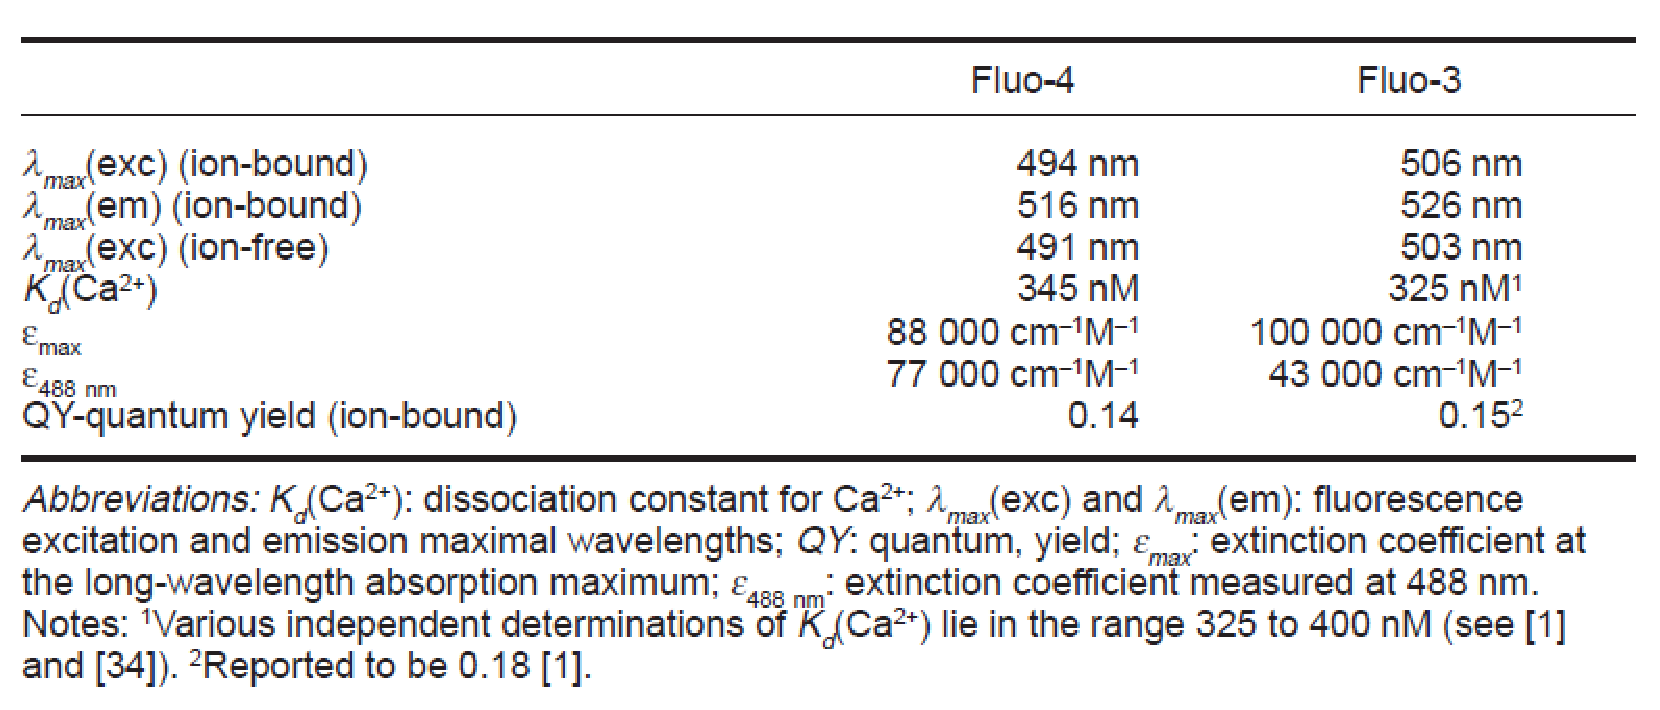
\includegraphics[height=5cm,
    angle=0]{./images/fluo-3_fluo-4.eps}}
  \caption{In vitro measurements of Fluo-3 and Fluo-4 properties}
  \label{fig:fluo-3_fluo-4}
\end{figure}


%
% \subsection{Challenges}
% \label{sec:challenges}

Accurate measurement of free $[\ca]_i$ is challenging for several
reasons~\citep{bassani1995a}
\begin{enumerate}
\item incubation of the dyes using
acetoxymethylester (AM) forms has not been scatter uniformly, i.e.
compartmentalization during loading can be significant. Typically, we need to
wait for a certain time (e.g. 15mins) for the dyes to diffuse uniformly.

\item indicator loading into the mitochondria, which occupy a
  significant portion of the cardiac cell (20-36\%) can be
  substantial

\item hydrolysis of AM can lead to $\Ca$-insensitive fluorescence, and
  consequently, underestimate $[\ca]_i$
\end{enumerate}


%
% Recently, estimation of fluorescence intensity has been reported, not based on
% $[\Ca]$, but using pseudoratio $\Delta F/F$
% \begin{equation}
% \Delta F/F  = \frac{F-F_\base}{F_\base-B}
% \end{equation}
% where F is CaF, $F_\base$ is the Ca-bound fluoresence intensity before
% stimulation, $B$ is the background signal (averaged of areas adjacent to the
% cell). $\Delta F/F$ is thought to approximately reflect $[\Ca]_i$ if there is no
% % change in dye concentration, intracellualr environment, or path length.

\subsubsection{Sheu-Sharma-Banerjee (1984) - Quin-2}
\label{sec:calibrate_Quin2}

\citep{sheu1984} defined F as the dynamics level of fluorescence in Quin-2
loaded cell. To detect $F_\max$, they increase $[\Ca]$ by disrupting the plasma
membrane using 70$\muM$ Digitonin. $F_\min$ is the auto fluorescence of the dye
itself, i.e. measured at $[\Ca] < 10$nM. To do so, they added 25mM EGTA at
pH=8.7 to take all Calcium ions. So, the level of free calcium is back
calculated using
\begin{equation}
[\Ca]  = K_d \frac{F - F_\min}{F_\max - F}
\end{equation}
with $K_d = 0.115\muM$. So result lead to $[\Ca] = 181\pm 18$ nM in resting
cell.

\subsubsection{Williams et al. (1990) - EGTA}
\label{sec:calibrate_EGTA}

Free calcium concentration can be estimated using
\begin{equation}
[\Ca]_i = K_d \times \frac{[\text{Ca-EGTA}]}{[\text{EGTA}]}
\end{equation}
As free calcium concentration is very small (about $10^6$ times smaller than
total $[\Ca]$), the above formula can be estimated as
\begin{equation}
[\Ca]_i = K_d \times \frac{[\text{solution B}]}{[\text{solution A}]}
\end{equation}
with solution B contains 10 mM Ca-EGTA, and solution A contains 10 mM EGTA.

\citep{williams1990} claimed that using the above formula having many sources of
errors. So, it's better to use indicators with dual excitation wavelength.

\subsubsection{Williams et al. (1990) - Fluo-3/Fura-2}

\citep{williams1990qic} used 2$\muM$ Fluo-3 and 0.5$\muM$ Fura-2 incubated for
10mins, leading to 42-175$\muM$ Fluo-3 and 13-27$\muM$ Fura-2 in the cell. The
experiments was done at room temperature (20-22$^\circ$).

MRC-500 confocal microscope coupled to Olympus IMT-2 inverted microscope and
oil-immersion lens NA=1.3.
The theory minimum thickness is 0.26$\mum$ in Z-plane resolution, though the
practical value is around 0.5$\mum$.

A line-scan image has dimension 768pixels $\times$ 128 lines repeated every
250ms. The intensity at each pixel is measured 6ms/line. The degree of
enhancement of Fluo-3 is defined as $F_\max/F_\min$ with $F_\max, F_\min$ are
fluorescence of calcium-bound dye under saturating $[\Ca]$ and $[\Ca]=0$ ($<
10^{-9}$M). The ratio was estimated 4.95$\pm$0.04 (so we can take $F_\max=4.95,
F_\min=1.0$).
The result also shown the propagation of $\Ca$ waves starting from the edge of
the cell is about 87$\mum/$sec, and starting from the center of the cell is
about 115$\mum/$sec (measured the slope).

\begin{equation}
\begin{split}
[\Ca] &= K_d \frac{[\CaF]}{[F]} \\
[F]   &= [F]_T - [\CaF]
\end{split}
\end{equation}
For the resting $[\Ca]$, then CaF/F$_T$=0.36. Thus, F/F$_T$=0.64. The
fluorescence intensity (increase from the resting level RL of value 122
grey-scale-unit to the stimulated level SL = 170 units) is the sum
of Ca-bound dye and the free dye
\begin{equation}
\text{RL} = F_\max \times [\CaF]/[F]_T + F_\min \times [F]/F_T = 2.42 \text{
intensity units}
\end{equation}
They detected the increase in intensity about 1.40, so SL = 2.42x1.4=3.39
(intensity units).


\subsubsection{Cheng et al. (1993) - Fluo-3}
\label{sec:cheng-et-al_subsect}

To convert nonratiometric signal into $[\Ca]_i$, ~\citep{cheng1993cse}
used the pseudoratio equation (Sect.\ref{sec:spark_cheng1993})
\begin{equation}
  \label{eq:1455}
  [\Ca]_i = K_d \frac{R}{\frac{K_d}{[\Ca]_{rest}}+1-R}
\end{equation}
with R=F/F0 is the emitted Ca-bound fluorescence divided by the resting
emitted fluorescence; each after background
subtraction. $[\Ca]_{rest}=100$nM, $K_d=1100$nM.

\subsubsection{Lipp-Niggli (1994) - Fluo-3/Fura-red}
\label{sec:lipp_niggli}

\citep{lipp1994} used a mixture of two $\Ca$ indicators with excitation spectra
in the visible range of wavelengths. Fluo-3 excite at 514nm with an increase in
green fluorescence (525nm) upon $\Ca$-binding; and the other Fura-red showed a
decrease in the red fluorescence (600nm). The ratio of the two fluoresecence can
be used to calibrate free $[\Ca]_i$ concentration.

The cell is loaded with 100$\muM$ Fluo-3 and 100$\muM$ Fura-red.

\subsubsection{Cannell-Cheng-Lederer (1994)}
\label{sec:cannell-cheng-lederer_1994}

Based on \citep{grynkiewicz1985} approach, the free $[\Ca]_i$ is calculated from
the observed fluorescence
\begin{equation}
\label{eq:1599}
[\Ca]_i = K_d \frac{\F -\F_\min}{\F_\max - \F}
\end{equation}
with $K_d$ is the affinity of the dye to $\Ca$, $F_\min$ is the fluorescence in
the absence of calcium ($[\Ca]_i=0$), and $\F_\max$ is the fluorescence in the
saturation of $\Ca$.

NOTE: For Fluo-3, $\F_\min \approx 0$, and $\F_\max$ can be estimated from the
resting level of $[\Ca]_i \approx 100$ nM.
\begin{equation}
\F_\max = \F_\rest \left( \frac{K_d}{[\Ca]_\rest} + 1 \right)
\end{equation}

If we use the normalized fluorescence R=F/F$_\rest$, then
\begin{equation}
[\Ca]_i = \frac{K_dR}{K_d/[\Ca]_\rest - R + 1}
\end{equation}

\subsubsection{Trafford et al. (1999) - Fluo-3}
\label{sec:trafford-et-al-99}

The free $[\Ca]_i$ is calculated from the observed fluorescence
\begin{equation}
\label{ eq:1499}
[\Ca]_i = K_d \frac{\F}{\F_\max - \F}
\end{equation}
with $K_d = 1035$nM.

\subsection{aequorin}
\label{sec:aequorin}

Aequorin is one of the first calcium indicators. They are bioluminescent
calcium-binding photoproteins (Ashley and Ridgway, 1968;
Shimomura et al., 1962).
\begin{itemize}
  \item  The first studies of $[\Ca]_i$ transient in Purkinje fibers were done by Wier et
al. \citep{wier1980, wier1982} using bioluminescent protein aequorin

Using aequorin and action potential, the signal of calcium transients consisted
of two components, L1 and L2, Fig.\ref{fig:Aequorin_L1L2}. L1 is the fast
component and L2 is the more slowly rising component. L2 occur after a brief
decline in luminescence. Except for the amplitude, L1 is quite constant for
different experimental conditions.  L2 can be removed indicated that the two
components have different underlying processes. L1 can be removed by using drug
D600 (which block LCC, but not NCX). Thus, it was hypothesized that L1 is due to
$\Ca$ entry via slow inward current ($I_\CaL$), and L2 is due to $\Ca$ release
from internal storage (SR). Using aequorin and Voltage-clamp,
Fig.\ref{fig:Aequorin_L1L2}(B), they observed the same phenomena:
L1 and L2.

  
\end{itemize}

The bioluminescence of aequorin is usually shown as $L/L_\max$
\citep{takahashi1999}. Previously, the relation between light (L) and $[\Ca]_i$
is nonlinear, with $L\approx [\Ca]_i^{2.5}$ in the physiological range
\citep{allen1977}.

\begin{equation}
L/L_\max = \left( \frac{1+K_R \times [\Ca]}{1+ K_{TR} + K_R \times [\Ca]}
\right)^n
\end{equation}
with $n$ is the number of $\Ca$-binding sites and $K_R, K_{TR}$ are equilibrium
constant for $\Ca$ binding to R state and transition between T and R states of
aequorin.


\begin{figure}[hbt]
  \centerline{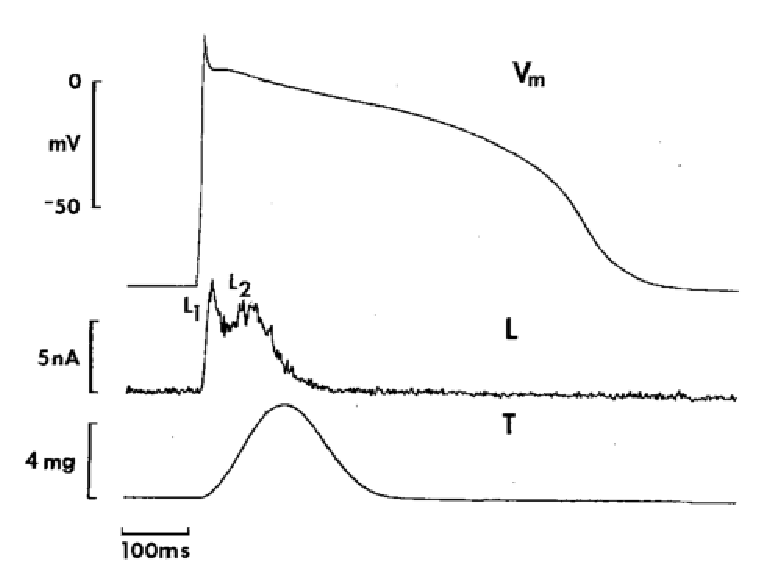
\includegraphics[height=5cm]{./images/Purkinjie_Calcium_Wier1982.eps},
  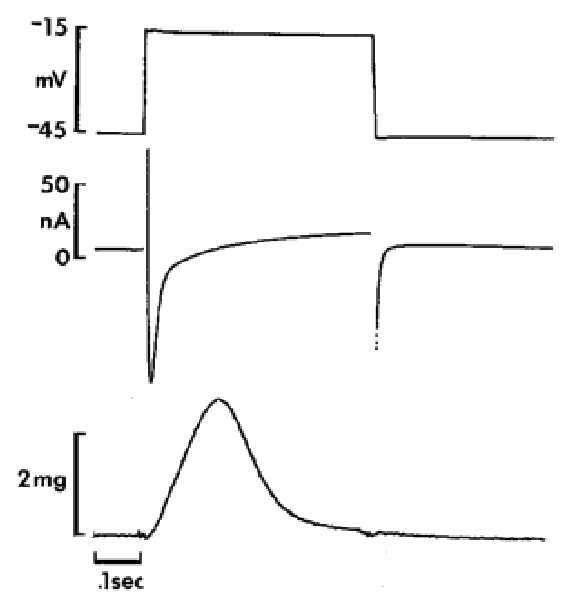
\includegraphics[height=5cm]{./images/LCC_current_Purkinje.eps}} \caption{AP
  (left) and V-clamp (right) experiment setting.
  {\bf Left}: Aequorin signal (L) associated with the action potential ($V_m$). 
  The contraction (T) reached peak within 130ms and completely relaxes within the
  200-300ms.
    {\bf Right}: from -45mV holding potential (to inactivate the fast $\Na$
    current) to -15mV for duration 500ms, frequency=every 2.5s}
  \label{fig:Aequorin_L1L2}
\end{figure}

\subsection{GFP-based $\Ca$ indicators}

For the case of GFP donor
\begin{equation}
[\Ca] = K_d \times (\frac{R-R_\min}{R_\max-R})^{1/n}
\end{equation}
with $n$ is the number of interacting sites of the indicators. Estimate minimum
and maximum values of fluorescence ratio $R_\min$, $R_\max$, and use {\it in
vivo} dissociation constant $K_d$

For the case of GFP acceptor
\begin{equation}
[\Ca] = K_d \times (\frac{F_\max - F}{F - F_\min})^{1/n}
\end{equation}

\subsection{Change in local SR}

Changes in local free $[\Ca]$ is derived based on Fluo-5N
(Sect.\ref{sec:fluo5N}).

\subsection{Level of calcium}


Resting calcium was estimated to be
\begin{enumerate}
  \item 0.05$\muM$ in cut fibers, and less than $0.06\muM$ in intact frog fibers
  \citep{kurebayashi1993}
  \item 0.18-0.27$\muM$ in intact frog fibers \citep{kurebayashi1993}
\end{enumerate}

The peak of $\Delta [\Ca]$ triggered by a single action potential was estimated
to be
\begin{enumerate}
  \item 20-30$\muM$ in cut fibers, and 10-15$\muM$ in intact frog fibers
  \citep{kurebayashi1993}
\end{enumerate}

\section{Laser line-scanning image}
\label{sec:confocal-line-scan}

The development of the fluorescent indicators was paralleled by the development
of new imaging instrumentation. A detailed discussion of imaging techniques is
discussed in Sect.\ref{sec:fluorecence_microscope}.  Here, we focus on
{\bf line-scanning confocal microscopies}. Other good books:
\citep{price2011bcm}.

The confocal microscope sequentially scans a focused point of light through the
specimen's fluorescent intensity at each spot. The brightness of individual
pixels in the line-scanning image is a representation of the fluorescence
intensity at the corresponding spot in the specimen, i.e. the summing of all the
photons coming from the area illuminated into a single value that become the
brightness value for that pixel.

The size of the smallest area can be detected as a single pixel has the radius
limited by the {\bf Airy disk}, i.e. the Airy disk define the smallest area can
be illuminated. The size of the pixel is assumed to be equivalent in size of the
excitation area in the specimen. The detector in laser-point scanning confocal
microscopes is {\bf photomultipler tube} (PMT), while that in spinning-disk
confocal microscope is the cooled coupled devices (CCDs). Here, spinning disk is
the disk containing an array of pinholes.

Higher N.A. lenses can collect photons count from wider angle. However, even
high N.A. lenses can collect maximum about 30\% of the emitted light. In a
well-maintained system with high quality optics, it's still doubtfull that
probably about 20-25\% of emitted photons will reach the detector
\citep{jerome2011dic}.

Laser-scanning confocal microscopy (Sect:\ref{sec:confocal-line-scan}) is better
than wide-field epifluorescence microscopy (Sect.\ref{sec:widefield_microscopy})
as it reduces out-of-focus fluorescence through defined optical sections inside
the specimens. It's the de facto for many research on calcium signalling and
cellular structure. However, it has the fundamental resolution limit (200-250nm
in lateral and 500-700nm in axial direction) \citep{Kohl2013} which is not able
to resolve many subcellular structure, e.g. mitochondria, RyR2 arrangement.
Newer imaging techniques include STED, RESOLFTs, SSIM, and techniques based on
localization of individual fluorescent proteins (STORM, PALM, FPALM)
\citep{Huang2009}.




\subsection{Mechanism}
\label{sec:mechanism-laser-scanning-confocal-microscopy}

There are two major platforms for laser scanning microscopy: confocal laser
scanning microscopy (cLSM) and multi-photon laser scanning microscopy (mLSM or
MPLSM) (two-photon or
three-photon)\footnote{\url{http://www.celanphy.science.ru.nl/Bruce web/scanning
microscopy.htm}}. The detection sides are DIFFERENT, but the illumination sides
are very similar. As shown in Fig.\ref{fig:LSM_diagram}, a beam of laser light
is focused into a small point at the plane called {\bf focal plane} (f.p.) of
the specimen, e.g. inside the cell loaded with a probe (e.g. fluorescence). The
scanning mirror is computer controlled to direct (move) the beam along the X-Y
direction at the focal plane. As it scans, the fluorescent emission at the focal
point on the focal plane  is detected by a {\bf photon multipler tube}. The
signal is reconstructed into an image using the computer hardware.

\begin{figure}[hbt]
  \centerline{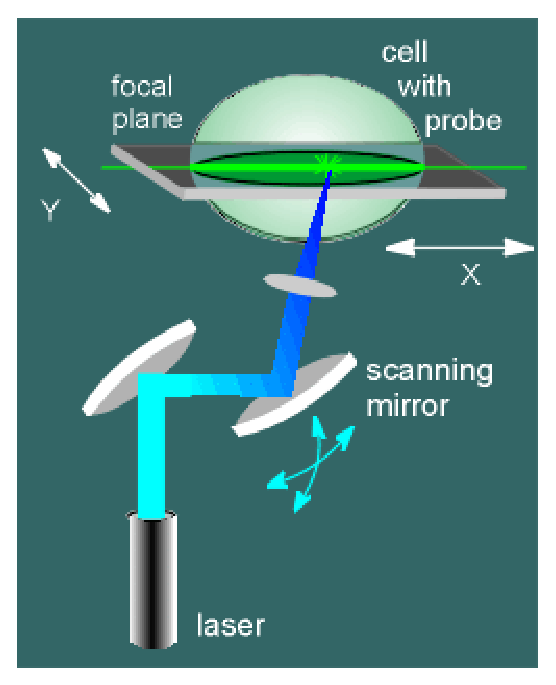
\includegraphics[height=5cm,
  angle=0]{./images/LSM_diagram.eps}}
  \caption{A schematic diagram of LSM}
  \label{fig:LSM_diagram}
\end{figure}

There are two modes of scanning, Fig.\ref{fig:LSM_modes}:
\begin{enumerate}
  \item {\bf X-t scans} (or line-scan imaging): the laser continually scans the
  same X-line through the specimen (at a fixed focal plane). Each scan give an 
 X-t line. These lines are stacked to give the temporal change of the signal
 along that line over time. There are several factors to determine the quality
 of the line-scan imaging: (1) the time to scan one line of a given length, (2)
 the pixel resolution. E.g.: To scan one line, BioRad MRC 600 or 1000 take 6ms.
 
 Conventionally, during confocal laser scanning, the data is acquired as the
 laser scans in only one direction. To improve the quality, 'bidirectional
 scanning' mode can be used \citep{hallett1999}. Data from one line is obtained.
 So the spatial information is very poor. 
 A better solution is X-Y scans.
 
  \item {\bf X-Y scans}: the laser light scan along the X-direction, then
  slightly move in the Y-direction, before doing another X-line scan. After the
  entire X-Y plane is scanned (one cycle), it goes back to the original location
  to start another X-line scan. Of course, it takes more time to complete one
  cycle, e.g. Biorad MRC 600 takes 400ms. So one cycle give the X-Y at a given
  time point. Multiple X-Y scans be saved as a stack of images. Each one give
  new information at every 400ms. Given a fixed speed of the detector, depending on the scan
  area (e.g. $128\times 128$ pixels or $512\times 512$ pixels), it may take
  shorter or longer to record an image, e.g. between 1.0 sec to 4.0 sec to
  record an image.
   
  \item {\bf X-Y-Z scan}: also possible, with the same mechanism. Due to the
  slowness, the method is rarely applied in dynamic imaging where time is
  important. However, the mode is very common in immunocytochemistry and other
  staining methods.
  
\end{enumerate}

\begin{figure}[hbt]
  \centerline{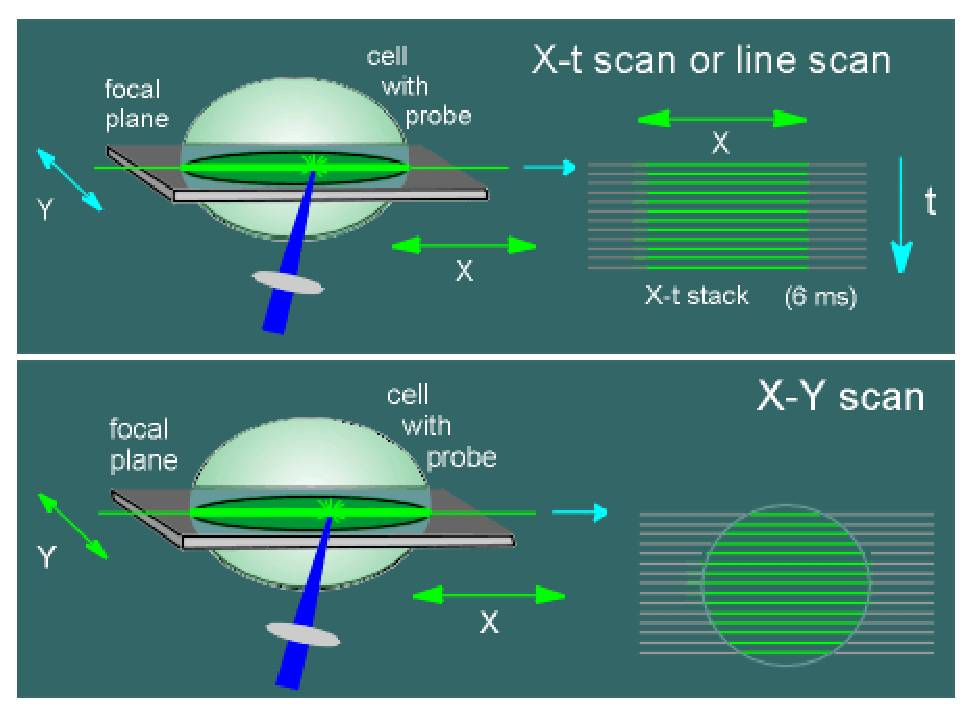
\includegraphics[height=5cm,
  angle=0]{./images/LSM_modes.eps}}
  \caption{Two modes of LSM}
  \label{fig:LSM_modes}
\end{figure}

In confocal laser scanning microscopy, the laser being used is (continuous) ion
laser, i.e. {\bf gas laser} (converting electrical energy to a laser light
output) that uses ionized gas. The most common ion is the mixed of Argon (Ar)
and Krypton (Kr), i.e. Ar/Kr, to give the output wavelength that appear as white
light. When the laser light, with high intensity, reflect on the specimen ($\Ca$
indicator or dye), it triggers the emission of fluorescent light (photons) on
the focal plane. However, considerable fluorescence is created above or below
the focal plane as well. To get rid of the out-of-focus light, a pin hole is
introduced to allow the detector (the photon-multiplier tube) to avoid the noise
as much as possible. As shown in Fig. \ref{fig:LSM_detection}, the light outside
the focal plane (i.e. the yellow in the figure) is largely excluded. Only the
light in the focal plane (i.e. the green in the figure) can pass through the pin
hole to reach the photon-multiplier tube. NOTE: The focus plane of illumination
is the same as the focal plane of detection, i.e. they are {\bf confocal}.

\begin{figure}[hbt]
  \centerline{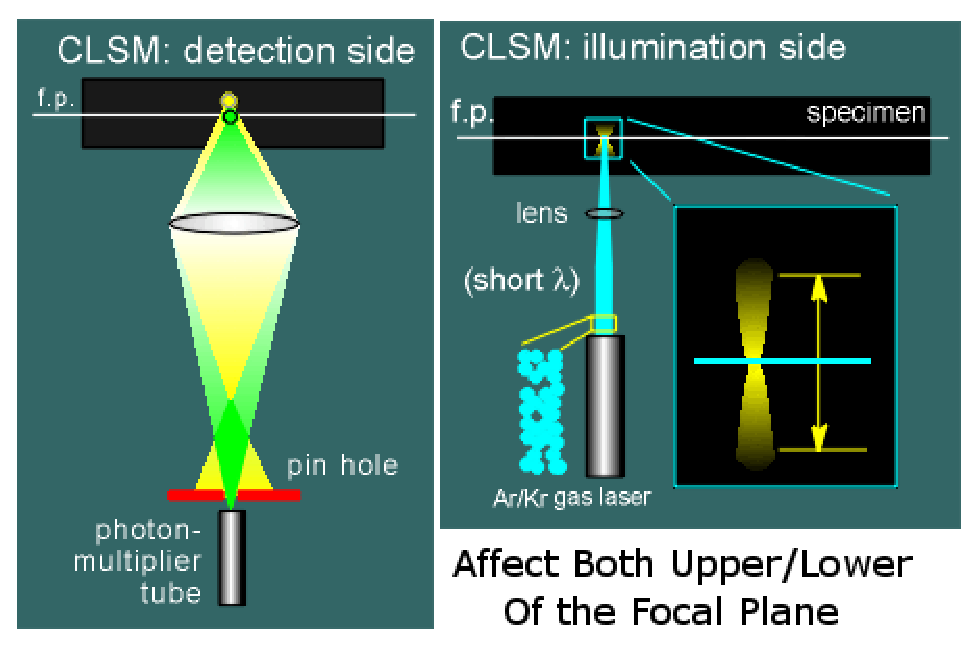
\includegraphics[height=5cm,
  angle=0]{./images/LSM_detection.eps}}
  \caption{Mechanism of detection of LSM}
  \label{fig:LSM_detection}
\end{figure}

In multi-photon laser scanning microscopy, the discrete lasers as {\bf solid
state laser} are used. Photons are given off in pulses, i.e. at some given
interval. A titanium sapphire laser (Ti:\ce{Al2O3}) can generate ultrashort
pulses, i.e. giving off photons at 10ns interval. Also, the wavelength can be
longer than that in gas lasers. Due to the dis-continuity of the signal, the
light energy reaching the probe is lower, Fig. \ref{fig:MLSM_mechanism}. When a
probe absorbs one photon from the first pulse of light, the electron is not
elevated completely to an excited state, but an intermediate or ``pseudo''
excited state. If only one photon is absorbed, the probe will fall back to the
ground-state (S0) without giving off any fluorescence. If, by chance, the second
photon (coming from the subsequent pulse of the laser) is absorbed, then the
electron of the probe is elevated to the true excited state (S1). Consequently,
fluorescent light will be given off for it to return to the ground state. The
chance to have two photons triggering the signal is higher in the focal-point
than out-of-focus points. This reduces out-of-focus signal dramatically. As
two-photon is required to excite, the system is called 2-photon laser scanning
microscopy \citep{helmchen2005}. An important advantage of MPLSM is that the
region excited by MPLSM is much smaller than that excited by CLSM,
Fig.\ref{fig:MLSM_mechanism}. 

\begin{figure}[hbt]
  \centerline{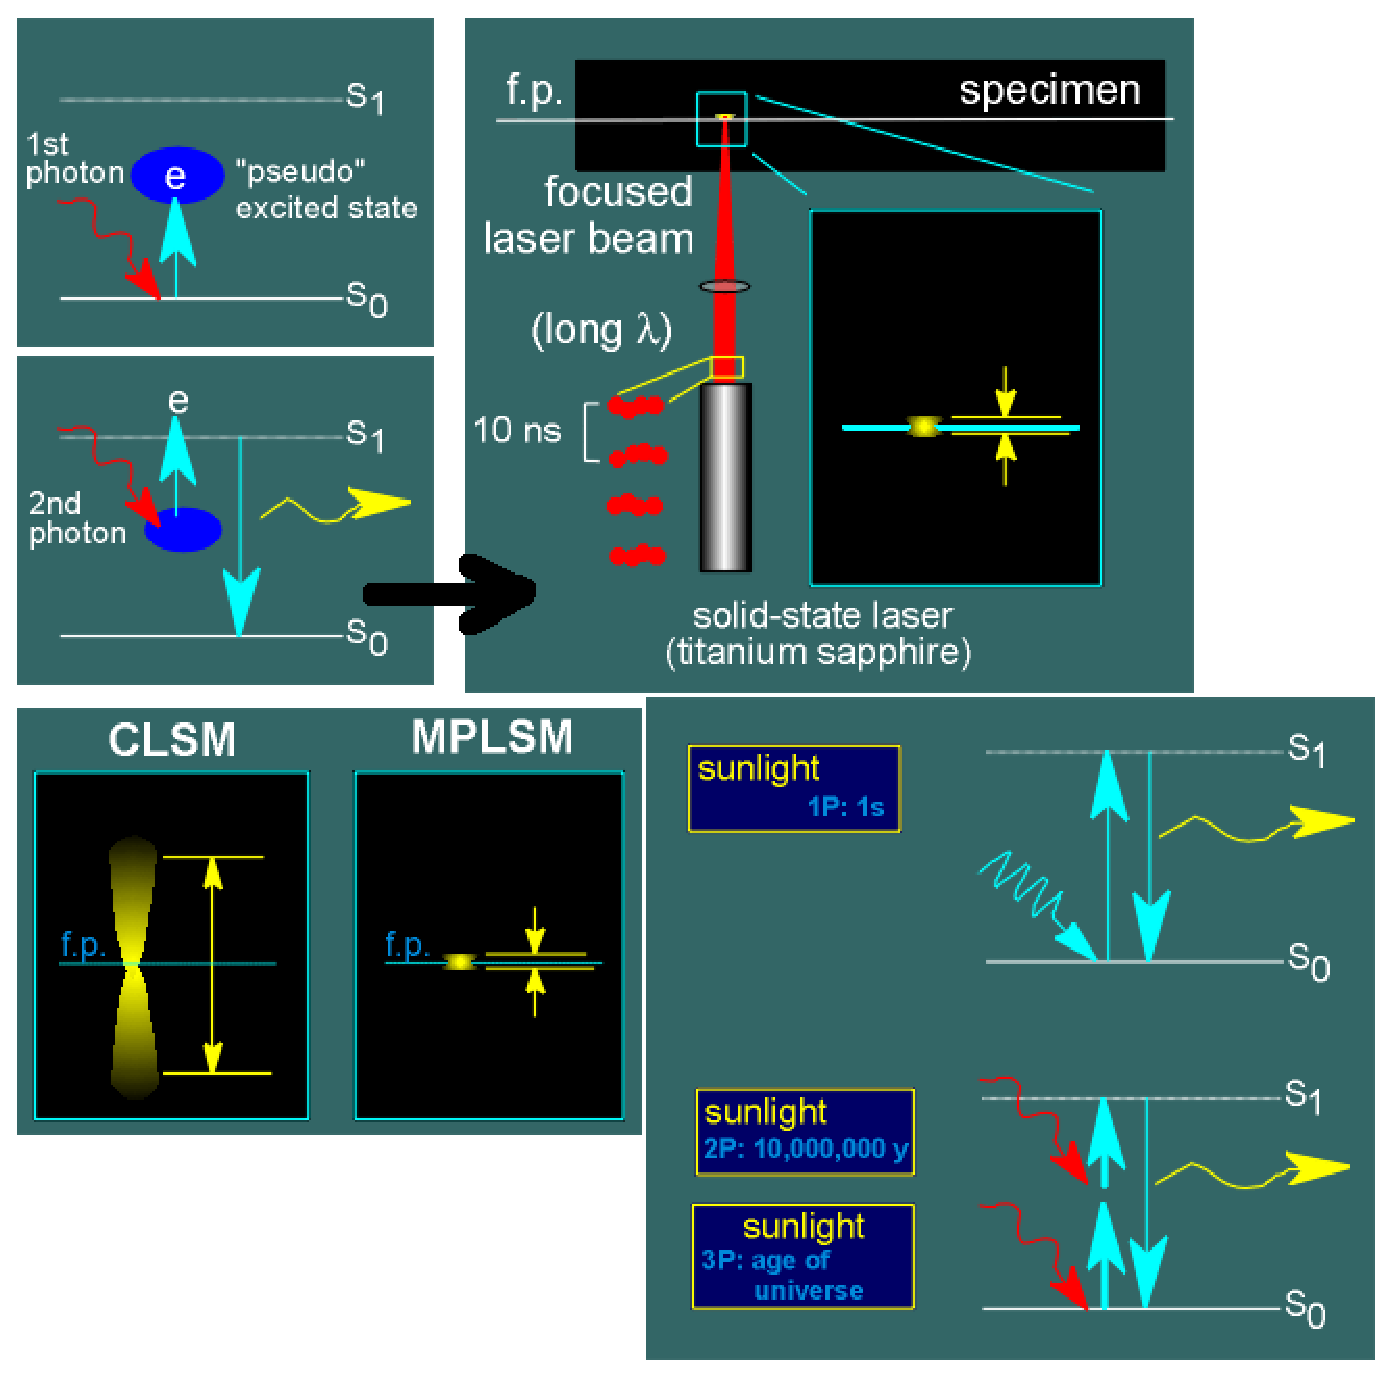
\includegraphics[height=7cm,
  angle=0]{./images/MLSM_mechanism.eps}}
  \caption{Mechanism of detection of MPLSM}
  \label{fig:MLSM_mechanism}
\end{figure}

\begin{framed}
The probability of multi-photon event is extremely low and occurs only where the
laser light is the most intense, i.e. at the focal point. An example: given the
laser light at the intensity of sunlight on earth, one-photon event occur once
every second, while two-photon event occur once every 10 million years. This
gives us the capability to detect event at a very small region. A three-photon
event is even more rare, occuring only once in the life time of the universe
at the intensity of the sunlight.  The laser beams generated by the microscopy
focusing at the very small poit has the intensity considerably higher than that
of sunlight. 

MPLSM is more sensitive than CLSM, thus giving a sharper image. The longer
wavelength being used in MPLSM is an advantage because it's inherently less
damaging to biological material than shorter wavelengths. Short-wave length in
CLSM is known to produce free radicals which can damage biological material. 
Also, longer wavelength can penetrate deeper (5x times) into biological material
(up to 500$\mum$ vs. 100$\mum$ for CLSM). This is important in imaging in
tissues.
\end{framed}

The $\Ca$-bound indicator reflects to the coming light and changes the light
wavelength. The emitted light, in terms number of photons, from $\Ca$-bound
indicator is recorded. Through the use of filters, only the wavelength
corresponding to the $\Ca$-bound indicator will be detected by the line-scanning
confocal light microscopy. In addition, the source light goes through a number
of filters to filtering away unwanted wavelengths, e.g.
out-of-focus wavelengths or wavelengths from the light emited by the free
indicator.

The intensity of this emitted light is captured by the CCD camera or can be
observed by human eyes. This intensity of fluorescence F(x,t) is directly
proportional to the concentration of free $\Ca$ (See calibration methods
Sect.\ref{sec:calibrate_Fluo}).
However, the correct estimation of free $[\Ca]$ from this intensity is highly
dependent upon the position of the confocal line-scan laser beam, the
linearity/non-linearity of the binding and the resolution of the microscopy
(diffraction limit).

\subsection{Line-scan images}

May articles have discussed these techniques: using Fluo-4
\citep{guatimosim2011}.

Cells are typically stimulated 1Hz for 15sec to reach steady-state condition
before recording. Line-scan image is recorded using ``X-t scans'' mode.
Typically, each image is a collection of about 512 lines, with interval $\sim
2$ms (skeletal cell), or 2.09 ms (cardiac cell). Each line is a collection of
768 intensities (pixels), taken at 0.139$\mum$ distances (skeletal muscle), or
0.156$\mum$ (cardiac cell). The fluorescence is normalized to the initial
intensity $F_o(x)$ which is obtained by averaging $F_o(x,t)$ before the
depolarizing pulse.
In confocal line-scannig microscopy (cLSM), the major problems with the
fluorescent imaging are {\bf photobleaching} and image  noise.

\begin{framed}
 Each fluorescent molecule can emit about $10^4-10^5$ photons/molecule before
 photolysis. However, when fluorescence is employed for imaging, the number
 is generally extreme small. So, the noise or statistical variation in the
 number of defected photons follows {\bf Poisson noise}.
 
 Photobleaching occurs when excessive excitation leads to the destruction of the
 fluorescent molecules and hence a reduciton in the emission intensity
 (bleaching). This is not the problem with ratiometric dyes as the ratio will
 remain the same, even when photobleaching occurs. With nonratiometric dyes,
 photobleaching can be reduced by attenuating the laser light, and increase the
 detector sensitivity (photomultiplier), yet it can increase the noise.
\end{framed}

To generate the original image (no noise, no optical blurring), a good
understanding of the nature of the image recording and processing of line-scan
images using cLSM is important. Ideally, one pixel on the image reflects the
intensity of one point source of a given size (fluorescent beads). However,
there are many factors that degrade the quality of the captured image, i.e.
causing optical blurring. So, energy emitted by a point source (fluorescence) at
the focal point captured by the objective lens is not as an equivalent pixel,
but rather a blurred set of diffraction fringes from the neighboring point
sources. The effect from farther pointsource is becoming less, and can be
modelled mathematically in the form of a {\bf point-spread function} (PSF).
Even though confocal modality was designed to reduce axial and lateral blurring,
it's never blur-free,
Fig.\ref{fig:psf_info}\footnote{\url{http://www.olympusmicro.com/primer/techniques/confocal/signaltonoise.html}}.
PSF has been known to be different in lateral direction (image plane x-y) and
axial direction (optical axis z).

\begin{figure}[hbt]
  \centerline{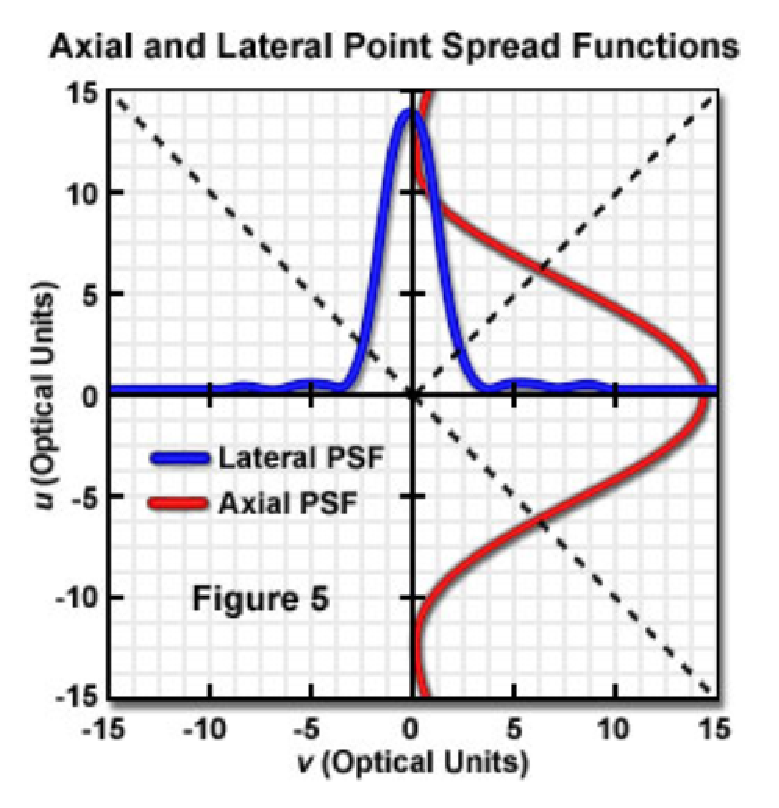
\includegraphics[height=5cm,
    angle=0]{./images/psf_info.eps},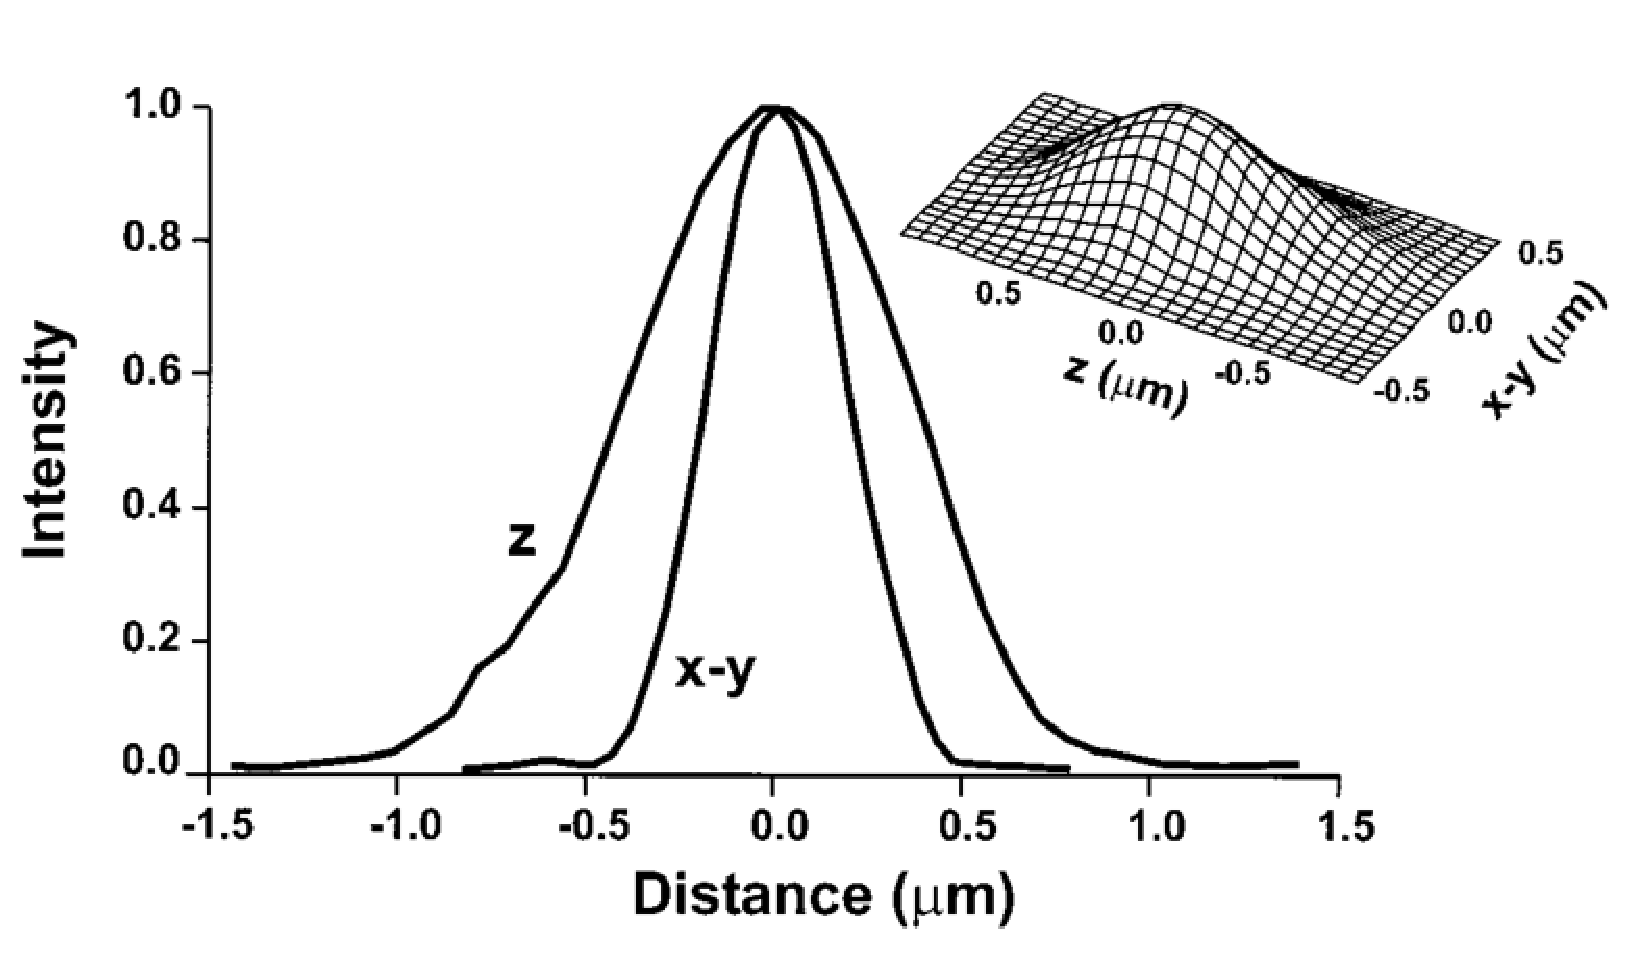
\includegraphics[height=5cm,
    angle=0]{./images/PSF_LSM410.eps}}
  \caption{(A) Axial and Later PSF; (B) PSF of 2-photon microscope with FWHM of
  400nm in x-y direction and 800nm in axial direction \citep{soeller1999}}
\label{fig:psf_info}
\end{figure}

The recorded (blurred) image can be represented mathematically by the equation
(replicated theoretically using a proper {\bf point-spread function} and
convolute with the simulated data).
\begin{equation}
\mathbf{g  = H \otimes (f + n)}
\end{equation}
with $\mathbf{g}$ is the blurred image (or the line-scanning confocal image).
$\mathbf{H}$ is the distortion operator, aka {\bf point-spread function} (PSF).
$\mathbf{f}$ is the ideal (unknown) raw picture, and $\mathbf{n}$ is the noise.
To find out $\mathbf{f}$, we need a good estimation of noise and PSF and then using
deconvolution operation. In a simulation scenario, as discussed in Sect.\ref{sec:artificial-line-scan}, we
have $f$ as the result of the simulation, we then need to apply  convolution,
using a proper PSF, adding some noise to give a computer-generated  line-scan
image $g'$. This image is expected  to be similar to what recorded from the
line-scanning confocal microscope.

\begin{framed}
The convolution of the function describing the actual light intensity
$i(x,y,z)$ with the point-spread function $\PSF(x,y,z)$ is described as
\begin{equation}
  \label{eq:1110}
  \begin{split}
  &\text{in 2D:} o(x,y,z) = i(x,y) \otimes \PSF(x,y) \\
  &\text{in 3D:} o(x,y,z) = i(x,y,z) \otimes \PSF(x,y,z)
  \end{split}
\end{equation}

\end{framed}

\section{Image enhancements}

Fluorescence was averaged over one to four pixels on both sides of the line
segment, at a rate of 30 frames/sec. Also, the baseline fluorescence $F_0$ was
defined as the background-subtracted fluorescence along the segment averaged
over 10 frames immediately preceding agonist exposure \citep{wang1993lpf}, e.g.
$\Delta F$ is avaraged in a 9 pixel-wide region of interest..

Image is represented using normalized fluorescence $\Delta F/F_0$.


\subsection{Noise}

The previous section (Sect.\ref{sec:mechanism-laser-scanning-confocal-microscopy}) has introduced the basic
mechanism of cLSM.  Given a simulated (or unknown) ideal image as input, where
the intensity of each pixel contains the number of photons (which could be
integer or floating-point).
\begin{enumerate}
  \item  For large number of photons, shot noise, with its Poisson
  characteristics, the standard variance is equivalent to the square root of the
  mean signal and behaves like Gaussian distribution.  Gaussian provides a
  symmetric (bell-shaped) curve prediciton of the distribution where x can be
  positive or negative. At high photon count, the estimation is  hard due to the
  power term in the distribution. So, Gaussian distribution is a  good
  approximation for the noise 
\begin{equation}
G_{\overline{x},s}(x,\overline{x},s) =
\frac{e^{-\frac{1}{2}(\frac{x-\overline{x}}{s})^2}}{s.\sqrt{2\pi}}
\end{equation}
 
  \item However, this is not correct when the number of photons is small.
  The measured fluorescence at each time at each pixel can be described by a
  signal plus correlated noise (SCN). In that scenario, the noise at each pixel
  scales with the intensity appropriately, not uniformly. So, A poisson noise
  model should be used.
  \begin{equation}
P_{\overline{x}}(x,\overline{x}) = \frac{(\overline{x})^x.e^{-\overline{x}}}{x!}
\end{equation}
Here, we only need to know the mean to estimate the distribution. IMPORTANT:
Poisson distribution requires x to be positive (i.e. the counting number).

  To remove the noise, digital deconvolution usig Richardson-Lucy algorithm is
  recommended \citep{richardson1972, vanderVoort1995, vankempen1997}. More
  detail: see \citep{soeller1999}.
  \begin{equation}
  I_{n+1}=I_n\left[ \frac{D}{I_n*H} \otimes H \right]
  \end{equation}
  with $D$ is raw data, $I_{n+1}$ is the revised image at step $(n+1)$. $*$ and
  $\otimes$ are convolution and cross-correlation operators, respectively. NOTE:
  15 iterations were used.
  
  In neuro sciences, approaches to processing two-photon data consist of
  averaging the measured fluorescence levels over multiple trials followed by
  kernel-based smoothing or fitting an appropriate curve to these time-series
  data (see \citep{malik2011}). To avoid using many data, principal component
  analysis (PCA) was also used to denoise the image data by dimension reduction
  \citep{mukamel2009}. Others used Fourier analysis of two-photon data from
  experiments of periodic stimulation to extract the signals at excitation
  frequency \citep{kalatsky2003, mrsic-flogel2003}, but not at other
  frequencies. \citep{malik2011} used harmonic regression to represent the
  signal and order $p$ autoregressive process to model correlated noise.
\end{enumerate}


\begin{framed}
Increasing the sample size give more accurate measurement of the number of
counts per sample, or the standard deviation decreases with sample size:
$s_{\overline{x}}=\sqrt{\overline{x}/N}$
\end{framed}

Changing the size of the focal spot of the confocal microscope at the specimen
results in a decrease number of photons detected, implying a higher noise level.
This is reflected via a smaller PSF. To maintain the same signal-to-noise, the
sampling period has to be increased which face the limitation capability of the
device itself. The effect of optical blurring caused by the diffraction limit
can be mathematically represented by applying 3D convolution with a point-spread
function will generate the theoretical 3D confocal image of $\Ca$-dependent
fluorescence. The captured signal (photons) is converted into the digital signal
by photomultiplier tube. By fixing z, we obtain a 2D confocal image, and by
fixing both z and y, we obtain a line-scan image.  Typically, 8-bit
photomultiplier is used, then saturated pixels (255)can be displayed in red or
yellow, while black-level pixels are displayed in blue or  greens.


Sect.\ref{sec:PSF} describes in detail point-spread functions (PSF).
Sect.\ref{sec:noise_confocalmicroscopy}. To generate a theoretical (confocal)
image, the result above need to be convolved in 1D, 2D or 3D space, at each
moment in time, with the measured PSF.

\begin{figure}[hbt]
  \centerline{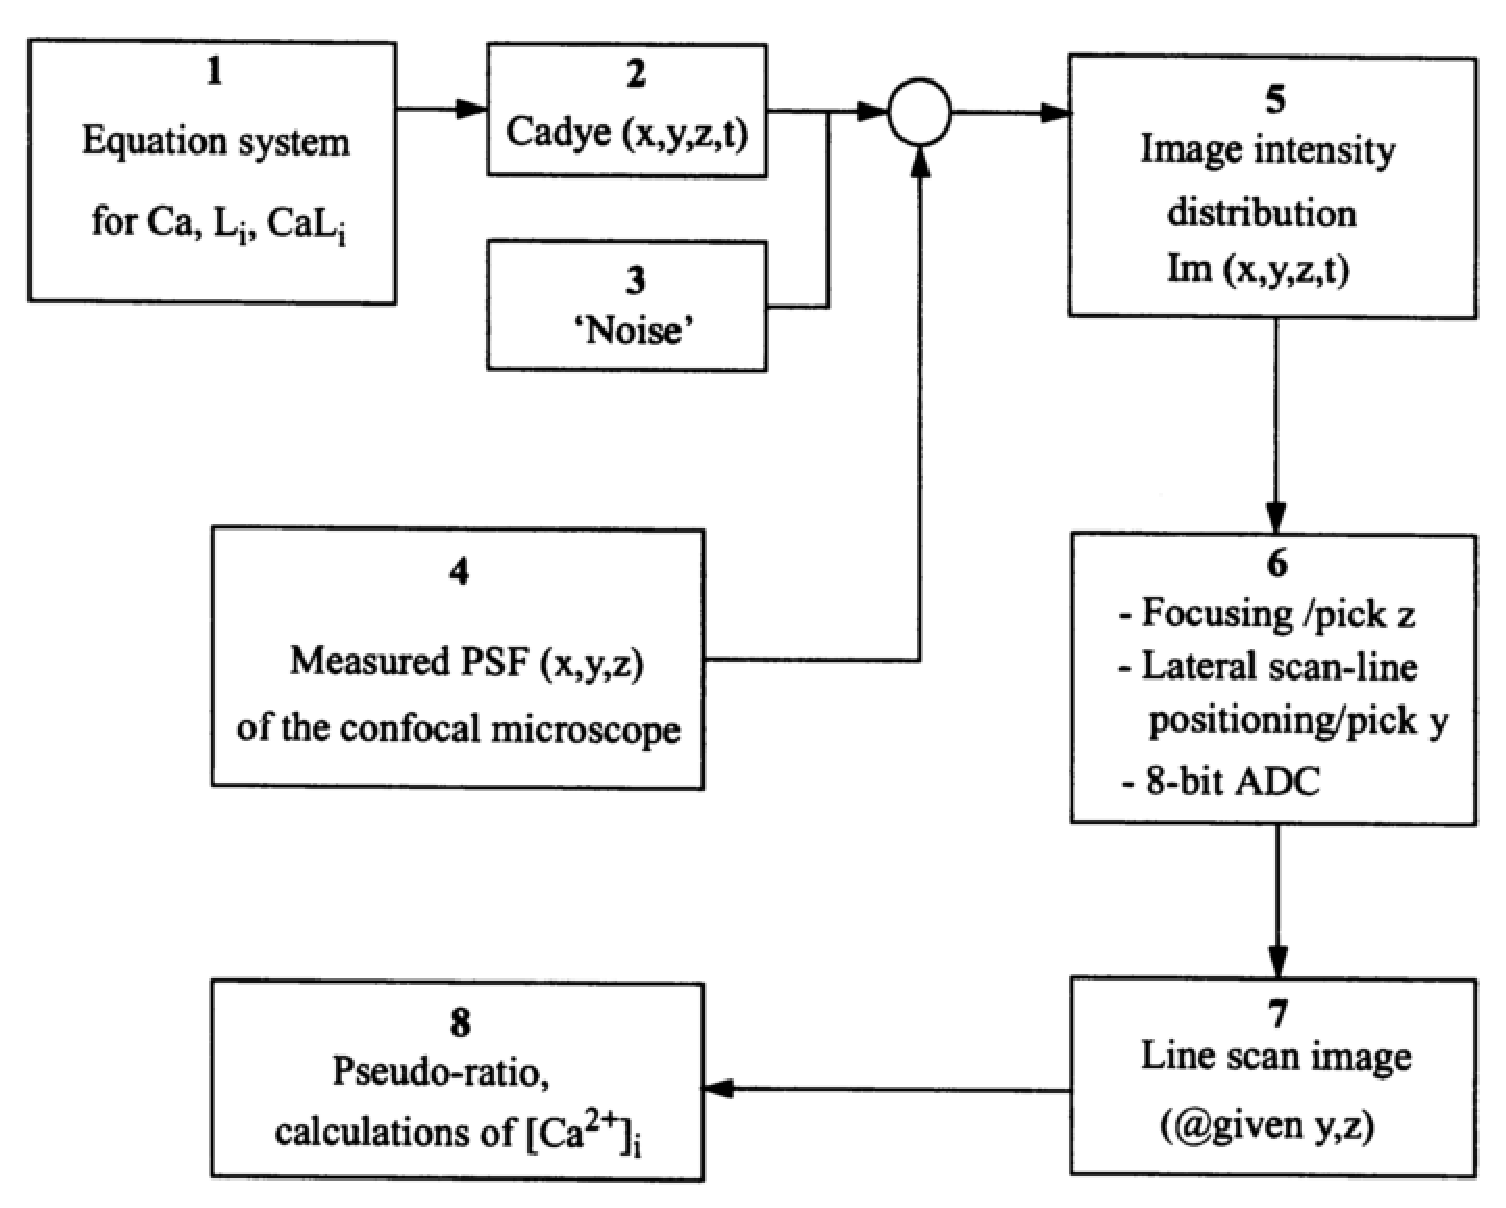
\includegraphics[height=7cm,
    angle=0]{./images/pratusevich_spark.eps}}
  \caption{$L_i$ represents the concentration of dyes and other
    intracellular buffers. $\ce{CaL_i}$ represents the concentration of
    Ca-bound form. The spatial distribution of Ca-bound form was
    convolved in 3D-space, at each moment in time, with a measured PSF
    to derive the image intensity. The direction of the scan line was
    assumed to be in parallel to the cell, $z$ is the direction of the
    optical axis of the microscope, $y$ is normal to the plane (x,z).}
  \label{fig:pratusevich_spark}
\end{figure}


Comparing between $\Ca$ sparks in intact myocytes and permeabilized myocytes,
the properties are similar, except the average amplitude are higher in intact
myocytes (0.905 $\Delta F/F0$ vs. 0.539 $\Delta F/F0$ based on criteria
$Cri=3.8$) \citep{picht2007}. Other parameters (FWHM, FDHM, full width, full
duration, and time to peak) are comparable for both conditions. Essentially,
$Cri=3.8$ is the standard choice for detecting sparks using automatic algorithms
\citep{cheng1999, picht2007}. If the noise level is low, and the amplitude of
the events is relatively high, we can use a smaller criteria, e.g. $Cri=3.2$.
The average full duration was 83.6ms (large events) and 38.6 (small events). The
average time constants from peak to nadir for small events was 19.7ms (fitted by
a single exponential function), and for large events was 42.2 ms (fitted by a
single expoential function; while using the sum of two exponential functions
give a smaller value for the time constant of the fast component 37.6 ms
\citep{gordienko2002}); average full width was 10.5 and 5.5$\mum$ in small and large events.

The smaller normalized amplitude $\Delta F/F0$ can be accounted by a higher free
$\Ca$ in the base-line (e.g. $[\Ca]_\myo$ = 150nM vs. 100nM) \citep{picht2007}.
The smaller spark amplitude in permeabilized vs. intact myocytes can be
explained by an increase in cytosolic $\Ca$ buffering capacity (due to 0.35mM
EGTA in the cytosolic solution).



\subsection{Devices}

\begin{framed}
The data format (.lsm) is a data format recording a line of laser point
scanning confocal or multiple-photon (two-photon) microscopes using Carl Zeiss
AG. The 5th generation of the device (Zeiss LSM 510, LSM 5 Pascal or LSM 5 Live)
is obsolete and should be replaced by the 7th generation (LSM 700, LSM 710 or LSM 780)
\end{framed}


Skeltal muscle, a device is used
\begin{enumerate}
  \item Microscope (Axiovert 100, Zeiss, Germany), with 40x, 1.2 N.A.
  water immersion objective (c-Apochromat, Zeiss) + inverted confocal microscope
  attachment to scan the fluorescence (MRC 1000, Bio-Rad, MA)
  \citep{cheng1999}, giving each pixel 2ms x 0.139$\mum$ (i.e. 512 lines/sec).
  
  \item MRC 1000 (Bio-Rad, Hercules, CA) with 40x, 1.2 N.A. water immersion
  objective (Zeiss, Germany), giving each pixel 2ms x 768 poins/line.
  Fluorescence F(x,t) was normalized to F$_o$(x), which is derived as average of
  F(x,t) before the depolarization pulse applied \citep{rios2001}, e.g. average
  data from 40ms to 20ms before the peak.
   
\end{enumerate}

Cardiac cell, a device is used
\begin{enumerate}
  \item Nikon Diaphot TMD with 60x, 1.4 N.A. oil-immersion objective + Bio-RAD
  MRC-600 confocal imaging system. The lens can move in the z-axis with a step
  of 0.02$\mum$, giving spatial resolution (i.e. PSF) FWHM$_{x,y}=0.48\mum$,
  FWHM$_z=1.30\mum$ \citep{pratusevich1996}. NOTE: PSF is measured by imaging a
  fluorescent bead 0.1$\mum$ in diameter, taking 16 optical sections along the
  z-axis with 0.28$\mum$ interval.
  
  \item Zeiss Plan-Nefluar 40x, 1.3 N.A. oil immersion objective + Zeiss LSM-410
  inverted confocal microscope, giving spatial resolution (i.e. PSF)
  FWHM$_{x,y}=0.5\mum$, FWHM$_z=1.0\mum$ \citep{song1997}.
  
  \item Inverted Epifluorescence microscope using $K_d=400$nmol/L
  \citep{trafford1997, dibb2004, walden2009}
 
  \item Zeiss LSM-410 inverted confocal microscope (Carl Zeiss, Inc., Germany),
  giving spatial resolution FWHM$_{x,y}=0.4\mum$,
  FWHM$_z=0.9\mum$ \citep{smith1998}, giving each pixel 2.0ms x 0.15$\mum$
  
  \item Microscope (Zeiss Plan-Neofluar) with 40x, 1.3 N.A. oil
  immersion objective + Zeiss LSM-410 inverted confocal microscope (Carl Zeiss,
  Inc., Germany), giving spatial resolution (i.e. PSF) FWHM$_{x,y}=0.4\mum$,
  FWHM$_z=0.9\mum$ \citep{cheng1999}, giving each pixel 2.09ms x 0.156$\mum$
  (i.e. 478 lines/sec).
  
  \item 63x, 1.4 N.A. oil immersion objective, giving spatial resolution (i.e.
  PSF) FWHM$_{x,y}=0.25\mum$, FWHM$_z=0.52\mum$ \citep{wier2000, izu2001lcg},
  giving each pixel 3ms (2.560ms for scanning and 0.440ms for flying 'back') x
  0.1$\mum$ (i.e. 256 pixels/line, 332 lines/sec). The photon count per pixel
  (with pixel duration 10$\mus$) typically not exceed 50 ( corresponding to a
  count rate of $5\times 10^6$ cps) \citep{izu2001}. The relatively small pixel
  size to ensure the Nyquist criterion is met. 
  
  \item Bio-Rad MRC 1024ES equipped with Olympus 60x 1.4 N.A. objective
  \citep{lukyanenko1999, lukyanenko2000, lukyanenko2001}. Using 30$\muM$ Fluo-3,
  each scan was digitized into 768 pixels/line, giving dimension each pixel of
  0.33$\mum$ x 6ms (i.e.
  166Hz). Amplitude F/F0 was determined using automatic algorithm
  \citep{song1997,cheng1999, lukyanenko2000}.

  \item Cat ventricular myocytes: confocal microscope (Radiance 2000/MP,
  Bio-Rad) \citep{picht2007}, giving 3ms x 0.12$\mum$ (i.e. 332 lines/sec). 
  
\end{enumerate}

Two-photon microscopy
\begin{enumerate}
  \item   Zeiss LSM 410 two-photon microscope: using Zeiss 63x, 1.25 N.A.
  oil-immersion objective. (X-Y)-Z images were obtained with a nominal spacing
  of 200nm along the optical axis. The spatial resolution FWHM$_{x,y}=0.4\mum$,
  FWHM$_z=0.8\mum$ \citep{soeller1999}. To exceed Nyquist criterion for image
  sampling, the voxel size was set to (x,y,z)=0.1x0.1x0.2$\mum$. The cell area
  that could be imaged is 102x102$\mum$.
  
\end{enumerate}

Video imaging
\begin{enumerate}
    \item Nikon Diaphot epifluorescence microscope 20x Fluor objective (Nikon),
  Hamamaatsu C2400 silicon-intensified target camera, Sony VHS video tape
  recorder: 1pixel = 0.86$\mum$ \citep{wang1993lpf}. 
    
\end{enumerate}

Fluorescence:
\begin{enumerate}
  \item Fluo-3 (Molecular Probes, Eugene, OR) \citep{cheng1999}, loaded 5$\muM$
  Fluo-3 AM for 5min \citep{walden2009}.
  \item 10$\muM$ Fluo-4 AM (Invitrogen) \citep{picht2007}
\end{enumerate}

\section{Automatic spark detection}
\label{sec:spark-detection}

Given the two types of $\Ca$ sparks, the first question is
\textcolor{red}{whether spontaneous sparks and evoked sparks really
  the same?}. Experimental data shown that it seems there is no significant
difference~\citep{cannell1995b,lopez-lopez1995}. Both transients reach the peak
in about 10ms. Then, the spark declines with half-time decay of about 20ms.
NOTE: The decline of global $\Ca$ transient is slower, about 160ms.

% \begin{enumerate}
% \item Sect.~\ref{sec:spark_cheng1993}
% \item Sect.~\ref{sec:collier-et-al}
% \end{enumerate}


The line-scan image can be F or $\Delta F/F0$. Typically, each pixel is of
dimension $0.139\mum$ and 2msec. Each line is typically 512 pixels length, i.e.
71$\mum$ (along the x-axis or the length of the cell). The PSF function is
typically FWHM$_{xy}=0.4\mum$ and FWHM$_z=0.9\mum$. The background noise at each
pixel should largely follow Poisson distribution.

\begin{framed}
Under voltage-clamp, the nature of raw image data is altered in 2 ways: 
\begin{enumerate}
  \item During the active clamp step, there may be a smooth elevation of
  background fluorescence
  \item there is a time interval, before the start of voltage clamp, during
  which there is a change in background noise is known to be present. 
\end{enumerate}
\end{framed}

Some studies reported modes in amplitude histograms \citep{tsugorka1995,
klein1996, lukyanenko1996, shirokova1997, xiao1997, satoh1997}. \citep{rios1997}
shown that calcium spark under voltage-clamp can have central mode. However, the
problem is complicated due to the unknown spark origin which can be at variable
distances from the scan line \citep{shirokova1997, smith1998}. Nevertheless, the
widely accepted theory of spark amplitude distribution is monotonic (without a
mode), i.e. each spark has only a single peak
\citep{pratusevich1996,smith1998,cheng1999}. Thus, the modes detected was
accounted by the bias in detecting against small amplitude events. Typically,
monotonic peak is the assumption. To detect spark peak from confocal image:
\begin{enumerate}
  \item $[\Ca]$ has to be at least 50nM  greater than $[\Ca]$ in neighboring
  region, time to peak in between 2 to 20ms, with half-time decay between
  10-40ms. The spatial FWHM at the peak from 0.5$\mu$m to 3$\mu$m
\end{enumerate}
To compare probability of sparks between trials (cells), we can normalized using
$P_s$=(number of spark)/(maximum number of sparks).

% \subsection{Spark characteristics}
% \label{sec:spark-char}
The wide variation in $\Ca$ sparks amplitude are assumed to be
affected by the two main factors:
\begin{enumerate}
\item positionally different (out-of-focus linescan position),
  i.e. the sensor doesn't point to the location of the peak calcium
  spark.
\item intrinsic different in CaRU properties, for which some release
  more $\Ca$ than others.
\end{enumerate}
To identify the affect of these factors individually,~\citep{izu1998}
studies the change (1) in RyR channel current or channel open time
which collectively called source strength $\alpha$, and (2) study the
$\Ca$ sparks amplitude histogram $N(\alpha)$
(Sect.~\ref{sec:izu-et-al}). Other factors to affect spark amplitude
are:
\begin{enumerate}
\item SR $\Ca$ load~\citep{satoh1997, gyorke1997, song1997}
\item different number of RyR openings in a spark~\citep{lipp1996}
\item SR RyR2 operate in subconductance mode, which then produce a
  different population of $\Ca$ spark with a smaller
  amplitude~\citep{xiao1997}.
\end{enumerate}


\begin{framed}
  \textcolor{blue}{Isopotential cell is a widely used assumption to
    model current flowing through a large population of voltage-gated
    ion channels}.
  In other words, at the same time, each channel experiences the same
  voltage and the activation of those channels experiences the same
  stochastic process. Hence, identical {\it rate constants} for gating
  mechanism can be applied to each channel and only average behavior
  needs to be considered.

  All the models developed in the first half of the book, including
  spatial models, use this assumption.
\end{framed}

Based on this monotonic assumption, \citep{cheng1999}
(Sect.\ref{sec:sparkdetect_cheng1999}) published the first and widely used open
source in IDL for automated spark detection.
\citep{picht2007} published the plug-in to work with ImageJ based on
\citep{cheng1999} algorithm. Another method developed for IDL by
\citep{sebille2005}. Previously, the process of identifying sparks from confocal
microscopy image is quite subjectively; with some arbitrary criteria, e.g.
minimum spatial half-width (i.e. full-width half maximal (FWHM)), amplitude
threshold, decay half-time. The algorithm of \citep{cheng1999} was based on the
idea (1) searching for connected regions that are above the noise level, (2)
once a spark is detected, the region is excised from the image, and use the new
image for repeating the spark analysis. To avoid recount the same spark that
have multiple peaks (because of noise). The threshold is \verb!Cri! or
\verb!Cri1!, and the criteria is usually $m+\text{Cri}\times \sigma$, with $m$
and $\sigma$ are mean value and standard deviation, respectively. From that, two
binary images (0 and 1) at levels of $m+2\sigma$ and $m+\text{Cri}\times \sigma$
are generated. NOTE: $m+\text{Cri1}$ is used in Voltage-clamp case. The
signal-to-noise is defined as $m/\sigma$. If we want to apply the noise to the
ideal image, we can adjust this ratio until a realistic look of the line-scan
image is obtained.


\subsection{Technical issues with spark magnitude detection}
\label{sec:techn-issu-with}

The fact that the image of a single point source is never a single
point, but a blurred and degraded finite area due to noise by the
imaging system.  In other words, if the object is an impulse function,
i.e. a single point with a given intensity, the result image is spread
out to form a finite area in the image plane (aka
{\bf Green's function} or impulse function). So, when the object is
divided into discrete point objects of varying intensity $O(u,v)$, the
image $I(x,y)$ is computed as a sum of the point-spread function (PSF)
of each source point. This process is usually formulated by a
convolution equation. Mathematically, the image is expressed as
\begin{equation}
  \label{eq:1033}
  I(x_i,y_i) = \int\int O(u,v) PSF(x_i-Mu,y_i-Mv)dudv
\end{equation}
with $PSF(x_i-Mu,y_i-Mv)$ is the image of the point with impulse
function $\delta(x_o-u,y_o-v)$.
\textcolor{red}{Knowing the correct PSF of the measuring device is
  very important in restoring the (original) image with
  deconvolution}.

% The image of the object can be seen as the convolution of the true
% object and a point-spread function (PSF).

% \begin{framed}
%   The output image is the convolution of the ideal image with the
%   PSF. The PSF is an impulse function. PSF can be constant or vary
%   over the plane field, depending on types of images. So, we need to
%   define zones of constant PSF (isoplanatic region) to allow use of
%   convolutional forms and the transform domain.
% \end{framed}

Using confocal line-scan image, it's not easy to detect the correct
peak of the $\ca$ spark, as we don't know the origin of spark relative
to the scan line. Other challenges are~\citep{pratusevich1996}
\begin{enumerate}
\item out-of-focus fluorescence
\item $\ca$ diffuse from the sites where it is released to the volume
  being observed
\item spatial-temporal profile of $\ca$ is different from that of the
  dye fluorescence
\end{enumerate}

The automatic way to detect sparks is based on the idea of detect
regions that have sufficiently high density of pixels with values
exceed some threshold level. The choice of the threshold is STD of the
background signal times a factor (e.g. 1.4) that can be varied by
users.
\begin{enumerate}
\item create a binary image, in which pixels in the images less than
  (background level + threshold) is set to 0; otherwise set it to
  unity.
\item detect high-density region of non-zero:
  \begin{itemize}
  \item at every pixel (i,j), the number of non-zero pixels within a
    square neighborhood of size N$_{size}$ centered on (i,j) is
    counted.
  \item if N$_{size}$ < N$_{live}$, then set (i,j) to zero (i.e. pixel
    ``dies''); otherwise set it to 1.
  \item Repeat the process N$_{generation}$ times for every pixel.
  \end{itemize}
  This can be implemented quickly using IDL. The number of living
  pixels for a single pixel can be found by using a boxcar averaging
  of size N$_{size}\times$N$_{size}$. Then, we threshold-setting all
  pixels to binary again using threshold as N$_{live}$. t

  The proper values: N$_{size}=7$, N$_{live}=12$ and
  N$_{generation}=3$ is good~\citep{izu1998}.
\end{enumerate}

\begin{framed}
  Before processing actual linescan images, the prominent horizontal
  lines seen in many images (see Fig. 1 A) are removed to avoid being
  identified as potential Ca2+ sparks by the detection program. This
  is done by setting the zero frequency component (corresponding to
  time) of the image's Fourier transform to zero. The linescan image
  without horizontal lines is recovered by inverting the modified
  transform.
\end{framed}



\subsection{Cheng et al. (1999)}
\label{sec:sparkdetect_cheng1999}

\citep{hollingworth2001} use this algorithm \citep{cheng1999}.

A 3x3 smoothed version of $\Delta F/F$ image was scanned for
possible sparks. Criteria: at least 3 consecutive pixels on a given scan line
and one contiguous pixel on the subsequent scan line has value $\Delta F/F$
greater than a threshold $\Delta F/F_\text{threshold}$.

F(x) is recalculated as average from F(x,t) after exclusion the region
identified as sparks (Sect.\ref{sec:sparkdetect_cheng1999}). Then,
recalculate $\Delta F/F(x,t)$ (eq.\ref{eq:1512}), and reapply the spark detection
again. The process is repeated until number of detected sparks and the points
associated with these sparks remain unchanged.


\section{Synthetic line-scan image}

To test the algorithms, we can generate synthetic images, i.e. the output not
from experiments nor from simulation. The peaks were varied from 0.05 to 0.70
(unit is $\Delta F/F0$), and signal-to-noise-ratio (SNRs) varying from 2.0
(high noise) to 4.0 (low noise).
\begin{equation}
\text{SNR} = \frac{\text{mean}}{\text{SD}}
\end{equation}
The amplitude of the synthetic spark ranged from 0.05 to 0.79 $\Delta F/F0$.
Also, the background level has the same mean of 38 (with standard deviation
(SD) of 19, 12.6, 9.5; corresponding to SNR of 2.0, 3.0 and 4.0). Typically, SNR
of $\sim 3$ was observed in both intact and permeabilized cardiomyocytes
\citep{picht2007}. This can be higher or lower, depending on the setting of
microscopes or experimental conditions. 



\section{Artificial line-scan image}
\label{sec:artificial-line-scan}

Concentration of Calcium-bound fluorescence, the output of a simulation, is the
data in Step (2), Fig.\ref{fig:pratusevich_spark} ~\citep{pratusevich1996}. To
generate an artificial line-scan image, we can follow the same protocol, i.e.
incorporate it with noise, and then do convolution with a given PSF. This
requires F and PSF to have the same overall dimensions and the voxels to be of
the same sizes.

The nature of the photon noise is Poisson, if the number of photons at each
pixel is high, we can approximate with Gaussian distribution, i.e. (in IDL)
\begin{verbatim}
img2 = 0L > ROUND( img1 + RANDOMN(seed, Nx, Ny)*SQRT(img1) )
\end{verbatim}
However, this is not correct when the number of photons per pixel is low. A
solution is
\begin{verbatim}
imnoise = POIDEV( im)

!or
imnoise =  randomn(im, /POISSON)

!or
a=3Drandomu(seed,poisson=3D10.0)
\end{verbatim}

A good, simple estimated PSF is the Gaussian kernel. Given that spatial
distribution of Ca2+-bound Fluo-3 is Gaussian, the spark is assumed to have
Gaussian profile. However, the recorded image doesn't show that.
The anisotropic of sparks can be explained (1) due to optical-blurring, or (2)
attributed to cellular structure and anisotropic diffusion rather than imaging.

\begin{framed}

A 2D PSF is isotropy due to the symmetric of the lens. However, in 3D, due to
the low resolution in axial, the 3D PSF is anisotropy.
The assumption of Gaussian $\Ca$-bound dye distribution is valid when the SR
  calcium release and the source strength is sufficiently weak so that the dye
  doesnot saturate. Then, we can assume PSF is Gaussian. So the convolution of a
  Gaussian Ca-bound dye concentration profile with a Gaussian PSF yields a
  Gaussian image.

  However, the observation image will deviate from Gaussian when the
  source is extended, or when the dye is saturated, or the confocal
  microscope is poorly aligned.
\end{framed}

The diffraction limited spots have shot noise (Poisson distributed) and
background noise (Gaussian distributed). So, to simulate data collected from a
fluorescence microscope, we use the following IDL
function\footnote{\url{https://groups.google.com/group/comp.lang.idl-pvwave/browse_thread/thread/604cab62a56a48ac?hl=en&pli=1}}.

The main source of noise is the photomultiplier tube, with the important
property that the level of the noise increases with increases in the level of
the signal. To model this noise, a normally distributed random variable was
added at each spatiotemporal point to the Cadye variable so that, for a given
point, the addition did not change the mean of the signal and the standard
variation was proportional to the mean. The proportionality coefficient (usually
0.5) was varied until the appearance of the resulting ratio images had been
adjusted to resemble a typical experimental record.

{\tiny 
\begin{verbatim}
FUNCTION psf, N, psf_width, bn_width, black_level, x_dim, y_dim, $
       x0, y0, Show=show
  ; psf generates a photon spot with background noise and
  ;  poisson noise.
  ; NOTE:
  ;      + psf_width is the stddev of the
  ;                  gaussian spot in units of pixels.
  ;      + bn_width is the stddev of the
  ;                 gaussian distributed background noise.
  ;
  ; Dan larson
  ; 5/22/00
;**********define the index arrays************************
x_dim = long(x_dim)
y_dim = long(y_dim)
array=lindgen(x_dim, y_dim)
xarr=array mod x_dim
yarr=array/x_dim

;**********define some parameters for the point spread function****************
F=1.0/(sqrt(2.0)*psf_width) ;This factor shows up repeatedly in the
                            ;error function calculation
a = 0.0
b = 0.0          ; a,b,c,d are transformed integration limits for the
                 ; error function
c = 0.0
d = 0.0
spot=dblarr(x_dim, y_dim)
poisson_noise=dblarr(x_dim, y_dim)
background_noise=bn_width*randomn(seed, x_dim, y_dim)   ; gaussian
distributed background noise with a black level
a=F*(yarr - 0.5 - y0)
b=F*(yarr + 0.5 - y0)
c=F*(xarr - 0.5 - x0)
d=F*(xarr + 0.5 - x0)
spot =N*0.25*(errorf(a)-errorf(b))*(errorf(c)-errorf(d))
index=where(spot GT 0, count)

;handle the case of no photons
if count gt 0 then begin
    location=array_indices(spot, index)
    for i=0, count-1 do begin
        poisson_noise(location[0, i], location[1, i])=randomn(seed,
poisson=spot[location[0, i], location[1, i]])
       ;if (photon GT 0.0) then poisson_noise(i-1, j-1)= randomn(seed,
poisson=photon) else poisson_noise(i-1, j-1) = 0.0; poissson
distributed shot noise
        endfor
    endif else begin
        poisson_noise=spot
    endelse
ideal_spot= black_level+spot
poisson_spot= black_level+poisson_noise
background_spot=black_level+background_noise

;********************this is the important spot**************
noisy_spot= black_level+background_noise + poisson_noise
if keyword_set(show) then tvscl, noisy_spot
;print, total(spot), total(poisson_noise)

A={ideal_spot:ideal_spot, poisson_spot:poisson_spot, $
      noisy_spot:noisy_spot, background_spot:background_spot, $
      spot_photons:total(spot), noisy_spot_photons:total(poisson_noise), max_noisy_spot:max(noisy_spot)}
return, A
end
\end{verbatim}
}

Although confocal modality has been designed to reduce axial and
lateral blurring, a confocal image is never blur-free. Each light
microscopic has a dimensionless optical point, so-called
{\bf point-spread function} (PSF).  PSF size is often expressed in
terms of the width at which the signal is of half the maximum
intensity (full-width half-maximum, or FWHM).

The shape of (unknown) PSF is an important factor in determining the
properties of the image. Thus, it's important the actual PSF to be
measured to analyze correctly the underlying formation process.
\begin{enumerate}
\item \citep{cheng1996csc} used FWHM 0.4$\mum$ in X-Y resolution, and 0.8$\mum$
in Z direction in images of 0.1$\mum$ fluorescent beads.

\item A typical lateral FWHM is $<0.4\mu$m~\citep{parker1997} and
  axial FWHM of 0.7-1.4$\mu$m for high power immersion objective lens
  in the focal plane~\citep{pratusevich1996}.

  E.g.: Using Nikon Diaphot TMD inverted microscope: the measured 3D
  PSF is highly asymmetric. The FWHM was 0.48$\mu$m in $y$-axis, and
  1.30$\mu$m in z-axis~\citep{pratusevich1996}.

\item ~\citep{smith1998} used {\bf point spread function} (PSF) as a
  3D Gaussian function having axial and lateral full width at
  half-maximum (FWHM) are different, i.e. 0.8$\mu m$ and $0.4\mu m$,
  respectively, comparable to the dimension of a $\ca$ spark
  (Sect.~\ref{sec:smith-et-al}).
  \begin{equation}
    \label{eq:971}
    G(x,y,z) = g(x,\sigma_{xy}).g(y,\sigma_{xy}).g(z,\sigma_{z})
  \end{equation}
  with $\sigma_{xy}=\frac{(0.4\mu m)^2}{(8 \ln2)}$, and $\sigma_z = \frac{(0.8\mu
    m)^2}{(8\ln2)}$. The values are based on the fact that $g(\text{FWHM}/2,\sigma)=g(0,\sigma)/2$
  \begin{equation}
    \label{eq:972}
    g(w,\sigma) = \frac{1}{\sqrt{2\pi\sigma}}\exp(-\frac{w^2}{2\sigma})
  \end{equation}


  So, the values of the pixels in the theoretical confocal line-scan
  image $[\ce{CaF}]_{avg}$ are calculated based on the simulated dye
  profile $[\CaF]$ as follows
  \begin{equation}
    \label{eq:970}
    \begin{split}
      I(x,Y_{offset},Z_{offset},t) &% [\ce{CaF}]_{avg}(x,Y_{offset},Z_{offset})
      = \\
      \int\int\int &[\CaF](x',y',z')\times G(x-x',Y_{offset}-y',
      Z_{offset}-z')dx'.dy'.dz'
    \end{split}
  \end{equation}
  with $Y_{offset},Z_{offset}$ represent the degree to which the origin
  of the spark is out of register with the center of the PSF, while $x$
  is the distance along the line scan.

\item ~\citep{izu1998} used also Gaussian function for PSF
  (Sect.~\ref{sec:izu-et-al})
  \begin{equation}
    \label{eq:1452}
    G(x,y,z) =
    N\exp(-\frac{x^2}{\sigma^2_{xy}})\exp(-\frac{y^2}{\sigma^2_{xy}})
    \exp(-\frac{z^2}{\sigma^2_{z}})
  \end{equation}
with $N=\frac{1}{\pi^{3/2}\sigma_{xy}^2\sigma_z}$ normalize the
integral of PSF over all space to unity. Similar to \citep{smith1998},
the standard deviation is related to FWHM as
\begin{equation}
  \label{eq:1453}
  \sigma=\frac{\FWHM}{2(\log(2))^{1/2}}
\end{equation}
with FWHM$_{xy}=0.4\mu$m, and $\FWHM_z=0.4...1.3\mu$m.

As both mobile Fluo-3 and immobile protein-bound Fluo-3 are
considered, the intensity of the image is the convolution of the
summation of the two function
% \begin{equation}
%   \label{eq:1451}
%   G_m(r,t) + G_i(r,t)
% \end{equation}
% as
\begin{equation}
  \label{eq:1454}
\begin{split}
  I ( x,Y_{offset},Z_{offset},t) = \int\int\int
  ([\CaFi](x,Y_{offset},Z_{offset},t) + \\
  [\CaFm])(x,Y_{offset},Z_{offset},t))
  G(x-x',Y_{offset}-y',Z_{offset}-z') dx'dy'dz'
\end{split}
\end{equation}

\item The PSF function of the microscope was determined by imaging 3-D
  stacks of 100 nm fluorescent latex beads in the medium used for
  mounting cells~\citep{soeller2008}
\end{enumerate}

The simulation result are often reported as $F/F_o$, by which it means
$[\CaF]_{avg}/[\CaF]_\infty$ where $[\CaF]_\infty$ is the resting
Ca-bound fluorescence (i.e. the one prior to depolarization)
\begin{equation}
  \label{eq:1119}
  [\CaF]_\infty = \frac{[\Ca]_\infty [F]_T]}{K_{d,F} + [\Ca]_\infty}
\end{equation}
and
\begin{equation}
  \label{eq:1120}
  \begin{split}
    [\CaF]_{avg}(x; Y_{offset},Z_{offset}) =\\
    \int\int\int [\CaF](x',y',z').G(x-x',Y_{offset}-y',Z_{offset}-z')dx'.dy'.dz'
  \end{split}
\end{equation}
with $G(x,y,z)$ is the PSF.

NOTE: The average fluorescence intensity (F, F0) can be measured in
whole-cell or for simplicity, we can take a small region of the cell,
e.g. over a 35$\mu$m wide region.

Although the intensity of the PSF extends in three dimension, typically we only
need to keep the lateral components (x and y), and we can neglect the axial
direction (z-depth). This 2D  lateral component is referred to as {\bf Airy
disk}. The resolution is directly related to FWHM of the PSF.


\begin{framed}
  The typical way to find the convolution is transforming to Fourier
  domain to map the convolution to multiplication, i.e. we find the
  discrete approximation of the Fourier transform of [CaF] and
  G($\cdot$), then we multiply them in the frequency domain. The size
  of the volume to carry out the convolution was dictated by the
  extent of the spreading of bound dye and the FWHM in axial and
  lateral direction.  Finally, the result is transformed back to the
  time domain.

  A typical volume (of $64^3$ elements) measure 3.6$\mu$m along the x-
  and y-directions and 4.5$\mu$m in the z-direction.
\end{framed}

$Y_{offset}, Z_{offset}$ is the line scan position on the y-z plane deviating
from the center of the release site, which is perpendicular to the x-axis. For
each time point $t_i$, we collect 1D array of $I(x,Y_{offset},Z_{offset},t_i)$ for all
x. Stacking all 1D array for all $t_i$, we form a line-scan image.

\begin{framed}
  A line-scan image is typically 256pixels per line (0.1$\mu$m per
  pixel), and 512 lines per frame (3ms per line). The small pixel size
  is required to ensure Nyquist criterion is met, as FWHM of the PSF
  of the microscope is 0.25$\mu$m~\citep{izu2001lcg}.
  ~\citep{izu1998} generated the line-scan image using 4$\mu$m in
  x-axis and 180ms in time.
\end{framed}

Recording a pixel is
\begin{enumerate}
  \item (1990-2000) typically 10$\mu$s for each pixel. So, recording a
line take 2.56ms, excluding 440$\mu$s for mirror ``flyback'', i.e. the
sensor returning to the original position to start a new line. Number
of photon counts per pixel typically not exceed 50 (counts per 10$\mu$s),
i.e. corresponding to a count rate of $50\times 10^5$ counts per
second (cps). Given the line-scan image of size 768pixels x 512 lines,
recording a line of 768 pixel take 768x10()$\mu$s)+440($\mu$s)=8.12(ms). So,
with 512 lines, it takes: 512x8.12=4,147(ms)=4.1(sec). 


  \item (2010+) typically takes 2$\mu$s in. So, recording a line (512 pixels)
  takes 1.54 (ms), including the flyback (about 0.2ms). Number of photon counts
  can be detected at a single pixel is about 30\%, i.e. the detection efficiency
  is about 30\%. A line-scan image is of 512pixels x 300 lines.
\end{enumerate}

Experimental data shown that the STD of the value in the recorded
image increase linearly (slope = 0.3) with the mean fluorescence, and
this relationship holds regardless of the sample region. So, to model
the noise,~\citep{izu1998} add a value to each simulated $I(x,y,z,t)$
point a random value from a Gaussian distribution with mean zero, and
$\sigma=0.3\times I(x,y,z,t)$.

``26-percent contrast of the Rayleigh criterion is considered reasonable in
typical fluorescence microscopy applications, and is the basis for the common
expression defining lateral resolution according to the following equation ``.

Line-scan images were typically 256 pixels per line, at 0.1 m per pixel, and
 512 lines per frame, at 3.0 ms per line. \citep{wier2000} recorded a line-scan
 image using a line of 25.6$\mum$ in length in 3ms. Of this
time, 0.44 ms are used for horizontal flyback. Thus the pixel dimension was
10$\mus$ and 0.1$\mum$. Long pixel duration limit the distance that can be
scanned. The peak of the pseudo F/F0 seldom exceed 4 or 5. $\Ca$ sparks with
F/F0 $\sim$ 2 can be detected experimentally.

The relatively small pixel size ensures that the Nyquist criterion is met,
because the FWHM of the point spread function (PSF) of the microscope is 0.25
$\mum$. Pixels are typically 10.0 $\mus$, giving time for linear scanning of
2560ms, with 440$\mus$ for ``mirror flyback'' of the reader. The number of
counts per pixel typically doesn't exceed 50, corresponding to a count rate of
$5\times 60$ cps.

\section{Generating spark profile}

There are two strategies: 
\begin{enumerate}
  \item extract a lines across the line-scan image (either
vertical or horizontal). This will allows us to detect time courses of spark at
different offset from the source (if using horizontal line), and the spark
spreading at different time point after the peak detected (if using vertical
lines). \citep{sobie2002tcas} in Fig.3(B) and (C), and Fig.4 middle trace.

  \item To find the FWHM and FDHM, we extract the region (4$\mum$ x 50ms) from
  the location of the spark. Then we extract a similar horizontal or vertical
  line, yet here for each line, we calculate the average all point along that
  line. \citep{sobie2002tcas} averaged over $1\mum$ wide (Fig.4 bottom trace).  
\end{enumerate}

\section{Softwares}

\subsection{Using ImageJ}

LSM image reader is now incorprated into ImageJ.

To isntall a new
plugin:\url{http://imagejdocu.tudor.lu/doku.php?id=howto:plugins:how_to_install_a_plugin}

Plugins: SparkMaster\url{http://sites.google.com/site/sparkmasterhome/home}

\subsection{Matlab - PsychoPhysics Toolbox}

Visual stimuli can be generated using Matlab's PsychoPhysics Toolbox.

\section{Experimental Techniques}

\subsection[SSV2008 - calcium mobility in SR]{Swietach - Spitzer - Vaughan-Jones
(2008) - SR $\Ca$ mobility}

A novel method to measure $\Ca$ mobility in the SR without using Fluo-5N loaded
into the SR. This avoids the effect of fluorophore (with $K_d=0.4$mM) enhancing
luminal $\Ca$ mobility as the Fluo-5 can functions as a mobile buffer.

In their method, $\Ca$ is drained slowly from SR by opening RyRs at one end,
using local exposure to caffeine. The method works well on both rat and guinea
pig, where Fluo-5N cannot be loaded reliably.

% \subsubsection{PSF (Optical blurringo)}
% \label{sec:optical-blurring}

